\documentclass[10pt]{article}
\usepackage[margin=0.7in]{geometry}
\usepackage{booktabs}
\usepackage{graphicx}
\usepackage{float}
\usepackage{hyperref}
\title{Formal Logic CoT Synthetic Results Update}
\date{2026-05-28}
\begin{document}
\maketitle

\section{Metric note for OOD benchmarks}
EM means exact match: after extracting explicit answer content from an \texttt{<answer>} tag or answer marker, the evaluator normalizes the prediction and gold answer and assigns 1 only when they exactly match, then averages over examples. GSM8K is numeric EM and is effectively an accuracy over single numeric answers, but the report does not fall back to arbitrary numbers elsewhere in a generated trace. For HotpotQA, 2WikiMultiHopQA, and MuSiQue the answers are free-form strings with aliases and partial-overlap possibilities, so the standard report is EM plus token-level F1 rather than calling the result plain accuracy. F1 gives partial credit for overlapping answer tokens; EM is the stricter all-or-nothing string match.

\section{Training sequence token lengths}
This audit uses the OLMo tokenizer over the actual SFT training mixtures. NL targets are longer than logic targets at every train range; total sequence lengths include the prompt plus target.

\begin{table}[H]
\centering
\small
\begin{tabular}{lllll}
\toprule
train range & logic target & NL target & logic total & NL total \\
\midrule
1..5 & 322 & 382 & 697 & 757 \\
1..10 & 500 & 653 & 1166 & 1319 \\
1..15 & 681 & 925 & 1637 & 1881 \\
1..20 & 863 & 1196 & 2109 & 2442 \\
1..25 & 1049 & 1469 & 2587 & 3008 \\
\bottomrule
\end{tabular}
\caption{Mean token lengths for main OLMo-7B SFT sequences by train-depth range.}
\end{table}

\section{Main OLMo-7B downstream OOD}
The broad OOD run has completed the 30-row main OLMo grid. This is downstream transfer under the strict answer extractor, not a synthetic validity score. The headline pattern is split: NL is much better on GSM8K numeric EM, while logic is much better on the context-provided multi-hop QA F1/EM tasks. Bold values mark the best value in each metric column.

\begin{table}[H]
\centering
\scriptsize
\begin{tabular}{lllllll}
\toprule
template & train max & n & GSM8K EM & Hotpot EM & 2Wiki EM & MuSiQue EM \\
\midrule
logic & 5 & 3 & 0.051 & 0.348 & 0.360 & 0.232 \\
logic & 10 & 3 & 0.072 & 0.360 & 0.338 & 0.228 \\
logic & 15 & 3 & 0.070 & 0.343 & 0.343 & 0.223 \\
logic & 20 & 3 & 0.079 & \textbf{0.383} & 0.348 & \textbf{0.247} \\
logic & 25 & 3 & 0.049 & 0.372 & \textbf{0.362} & 0.232 \\
nl\_exact & 5 & 3 & \textbf{0.491} & 0.147 & 0.172 & 0.083 \\
nl\_exact & 10 & 3 & 0.478 & 0.160 & 0.157 & 0.087 \\
nl\_exact & 15 & 3 & 0.322 & 0.193 & 0.183 & 0.115 \\
nl\_exact & 20 & 3 & 0.409 & 0.175 & 0.165 & 0.098 \\
nl\_exact & 25 & 3 & 0.256 & 0.127 & 0.132 & 0.078 \\
\bottomrule
\end{tabular}
\caption{OOD exact-match means over seeds for the main OLMo-7B checkpoints.}
\end{table}

\begin{table}[H]
\centering
\scriptsize
\begin{tabular}{llllll}
\toprule
template & train max & n & Hotpot F1 & 2Wiki F1 & MuSiQue F1 \\
\midrule
logic & 5 & 3 & 0.469 & 0.418 & 0.296 \\
logic & 10 & 3 & 0.478 & 0.401 & 0.295 \\
logic & 15 & 3 & 0.459 & 0.407 & 0.282 \\
logic & 20 & 3 & \textbf{0.504} & 0.409 & \textbf{0.312} \\
logic & 25 & 3 & 0.489 & \textbf{0.422} & 0.301 \\
nl\_exact & 5 & 3 & 0.198 & 0.202 & 0.113 \\
nl\_exact & 10 & 3 & 0.216 & 0.193 & 0.127 \\
nl\_exact & 15 & 3 & 0.251 & 0.229 & 0.161 \\
nl\_exact & 20 & 3 & 0.233 & 0.189 & 0.133 \\
nl\_exact & 25 & 3 & 0.175 & 0.163 & 0.099 \\
\bottomrule
\end{tabular}
\caption{OOD F1 means over seeds for the main OLMo-7B checkpoints. GSM8K is omitted because the task is scored by numeric exact match rather than answer-token F1.}
\end{table}

\subsection{Bare-format OOD rerun}
The format-matched bare rerun wraps the task content in \texttt{<question>...</question>} and lets the checkpoint emit its learned answer format. The 30-row main OLMo-7B slice is complete. Compared with the answer-only OOD run, NL remains much stronger on GSM8K, while logic remains stronger on context-provided QA.

\begin{table}[H]
\centering
\scriptsize
\begin{tabular}{lllllll}
\toprule
template & train max & n & GSM8K EM & Hotpot EM & 2Wiki EM & MuSiQue EM \\
\midrule
logic & 5 & 3 & 0.046 & 0.368 & 0.362 & 0.225 \\
logic & 10 & 3 & 0.043 & 0.373 & \textbf{0.363} & 0.238 \\
logic & 15 & 3 & 0.064 & \textbf{0.382} & 0.358 & 0.230 \\
logic & 20 & 3 & 0.066 & \textbf{0.382} & 0.362 & \textbf{0.245} \\
logic & 25 & 3 & 0.025 & 0.378 & 0.343 & 0.238 \\
nl\_exact & 5 & 3 & \textbf{0.369} & 0.223 & 0.237 & 0.130 \\
nl\_exact & 10 & 3 & 0.341 & 0.258 & 0.205 & 0.128 \\
nl\_exact & 15 & 3 & 0.287 & 0.210 & 0.195 & 0.117 \\
nl\_exact & 20 & 3 & 0.277 & 0.240 & 0.202 & 0.152 \\
nl\_exact & 25 & 3 & 0.242 & 0.113 & 0.093 & 0.063 \\
\bottomrule
\end{tabular}
\caption{Bare-format OOD exact-match means for the completed main OLMo-7B slice.}
\end{table}

\begin{table}[H]
\centering
\scriptsize
\begin{tabular}{llllll}
\toprule
template & train max & n & Hotpot F1 & 2Wiki F1 & MuSiQue F1 \\
\midrule
logic & 5 & 3 & 0.496 & 0.421 & 0.296 \\
logic & 10 & 3 & 0.501 & 0.424 & 0.309 \\
logic & 15 & 3 & 0.508 & 0.422 & 0.302 \\
logic & 20 & 3 & \textbf{0.509} & \textbf{0.426} & \textbf{0.316} \\
logic & 25 & 3 & 0.501 & 0.404 & 0.316 \\
nl\_exact & 5 & 3 & 0.305 & 0.281 & 0.177 \\
nl\_exact & 10 & 3 & 0.345 & 0.257 & 0.181 \\
nl\_exact & 15 & 3 & 0.288 & 0.249 & 0.169 \\
nl\_exact & 20 & 3 & 0.331 & 0.245 & 0.214 \\
nl\_exact & 25 & 3 & 0.147 & 0.112 & 0.082 \\
\bottomrule
\end{tabular}
\caption{Bare-format OOD F1 means for the completed main OLMo-7B slice.}
\end{table}

\begin{table}[H]
\centering
\small
\begin{tabular}{lllll}
\toprule
template & train max & seed & GSM8K EM & GSM8K tag \\
\midrule
logic & 20 & 3407 & 0.234 & 0.976 \\
nl\_exact & 20 & 3407 & \textbf{0.676} & \textbf{0.997} \\
\bottomrule
\end{tabular}
\caption{OLMo-2-32B bare-format GSM8K rerun. Full LongBench is intentionally skipped for this model because its configured context limit is 4096.}
\end{table}

\section{Main OLMo-7B HFSA result}
\begin{table}[H]
\centering
\small
\begin{tabular}{lllllllll}
\toprule
template & train max & n & OOD c@16 & OOD joint@16 & hard c@16 & hard joint@16 & d50 c@16 & d50 joint@16 \\
\midrule
logic & 5 & 3 & 0.293 & 0.052 & 0.207 & 0.013 & 0.135 & 0.010 \\
logic & 10 & 3 & 0.727 & 0.362 & 0.697 & 0.292 & 0.479 & 0.010 \\
logic & 15 & 3 & 0.634 & 0.293 & 0.675 & 0.372 & 0.354 & 0.042 \\
logic & 20 & 3 & 0.830 & 0.441 & 0.887 & 0.627 & 0.854 & 0.198 \\
logic & 25 & 3 & 0.921 & 0.710 & 0.956 & 0.839 & 0.833 & 0.417 \\
nl\_exact & 5 & 3 & 0.502 & 0.318 & 0.391 & 0.167 & 0.292 & 0.000 \\
nl\_exact & 10 & 3 & 0.482 & 0.299 & 0.425 & 0.221 & 0.417 & 0.000 \\
nl\_exact & 15 & 3 & 0.322 & 0.137 & 0.397 & 0.233 & 0.260 & 0.000 \\
nl\_exact & 20 & 3 & 0.474 & 0.219 & 0.649 & 0.479 & 0.406 & 0.115 \\
nl\_exact & 25 & 3 & 0.794 & 0.748 & 0.885 & 0.860 & 0.510 & 0.427 \\
\bottomrule
\end{tabular}
\caption{Final sparse-protocol means over seeds. Logic joint uses citation-free formal validity; NL joint uses translated NL-to-FOL validity.}
\end{table}

\begin{figure}[H]\centering
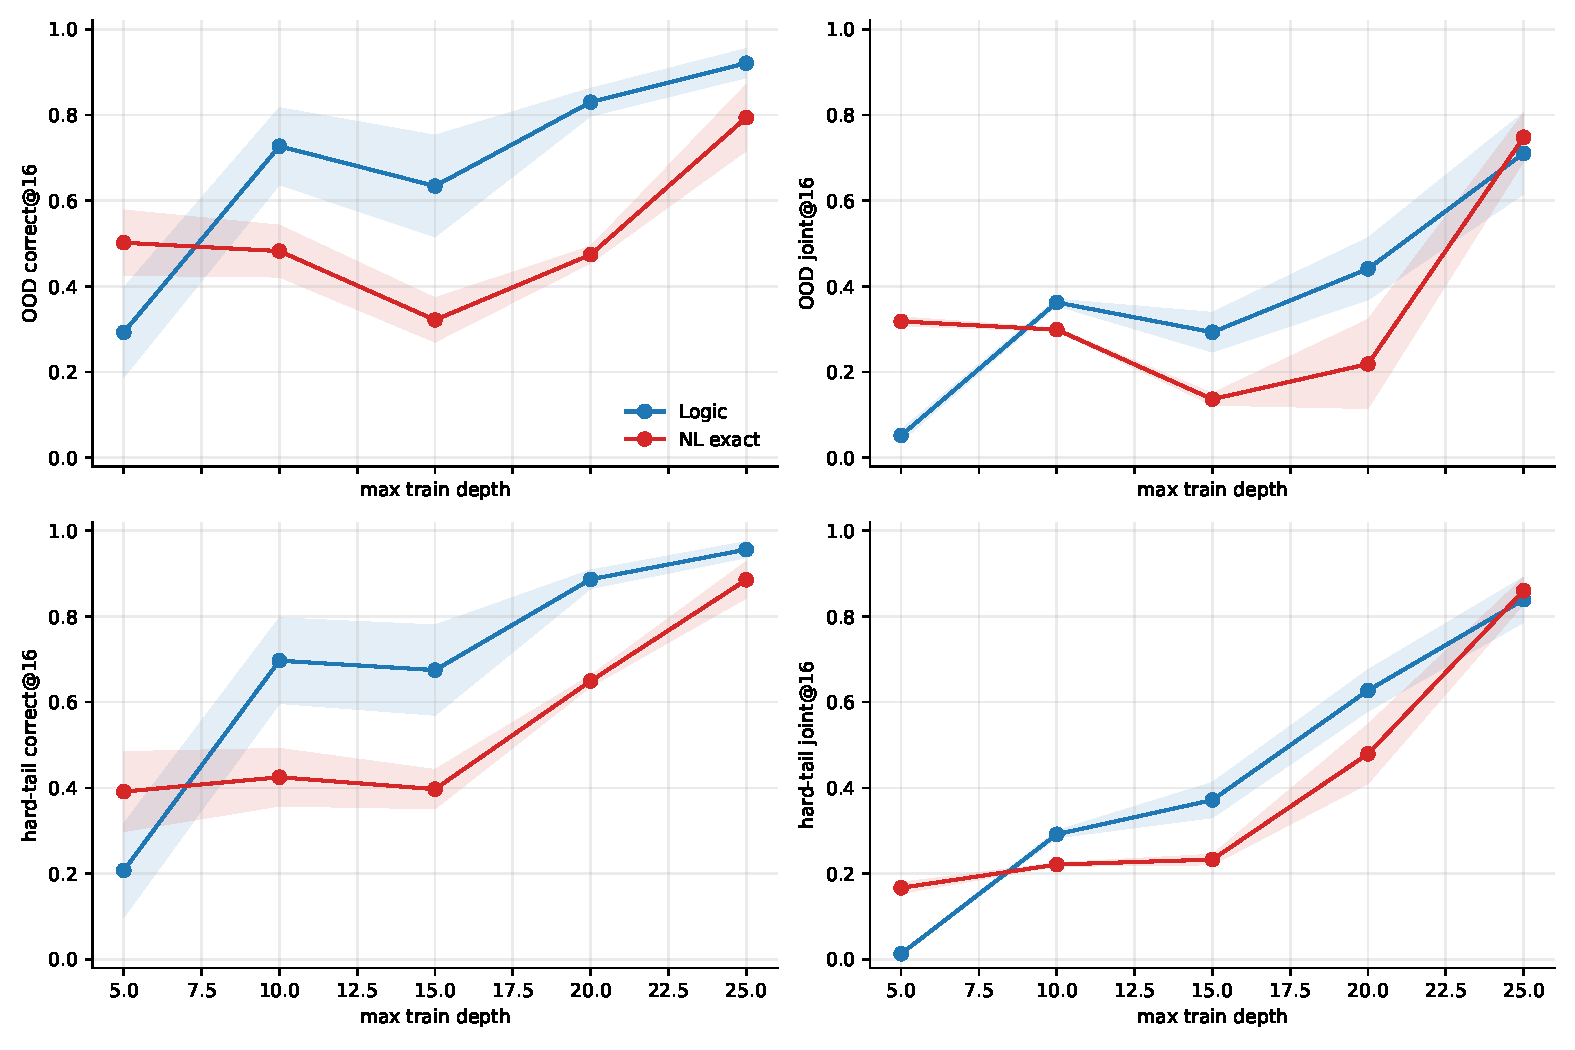
\includegraphics[width=\linewidth]{figures/olmo7b_final_by_train_depth.pdf}
\caption{Final OOD and hard-tail correct/joint performance as train depth increases.}
\end{figure}
\begin{figure}[H]\centering
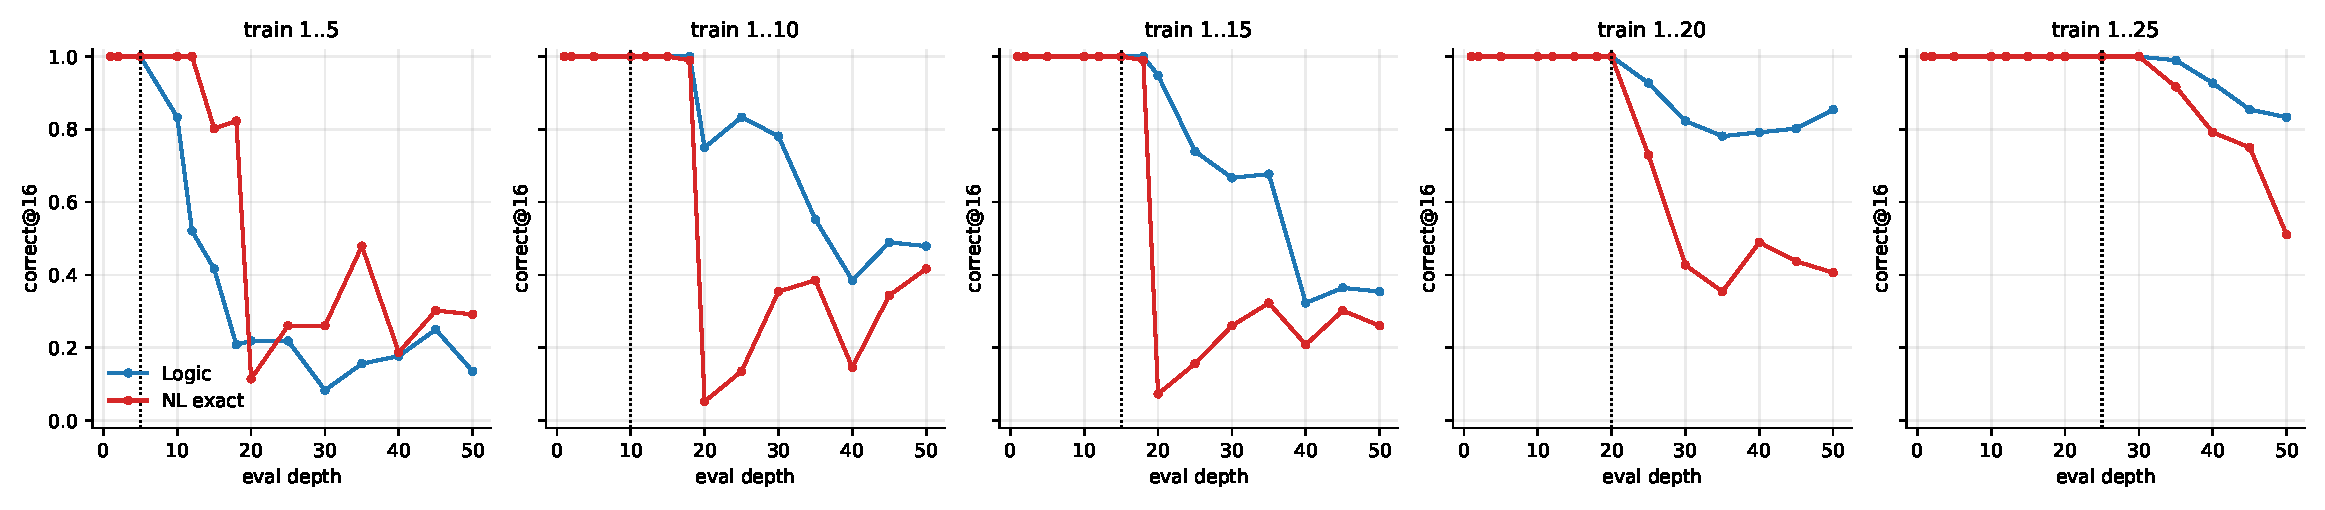
\includegraphics[width=\linewidth]{figures/olmo7b_depth_correct16.pdf}
\caption{Depth curves for final correct@16, averaged over seeds. Vertical dotted line marks the max train depth.}
\end{figure}
\begin{figure}[H]\centering
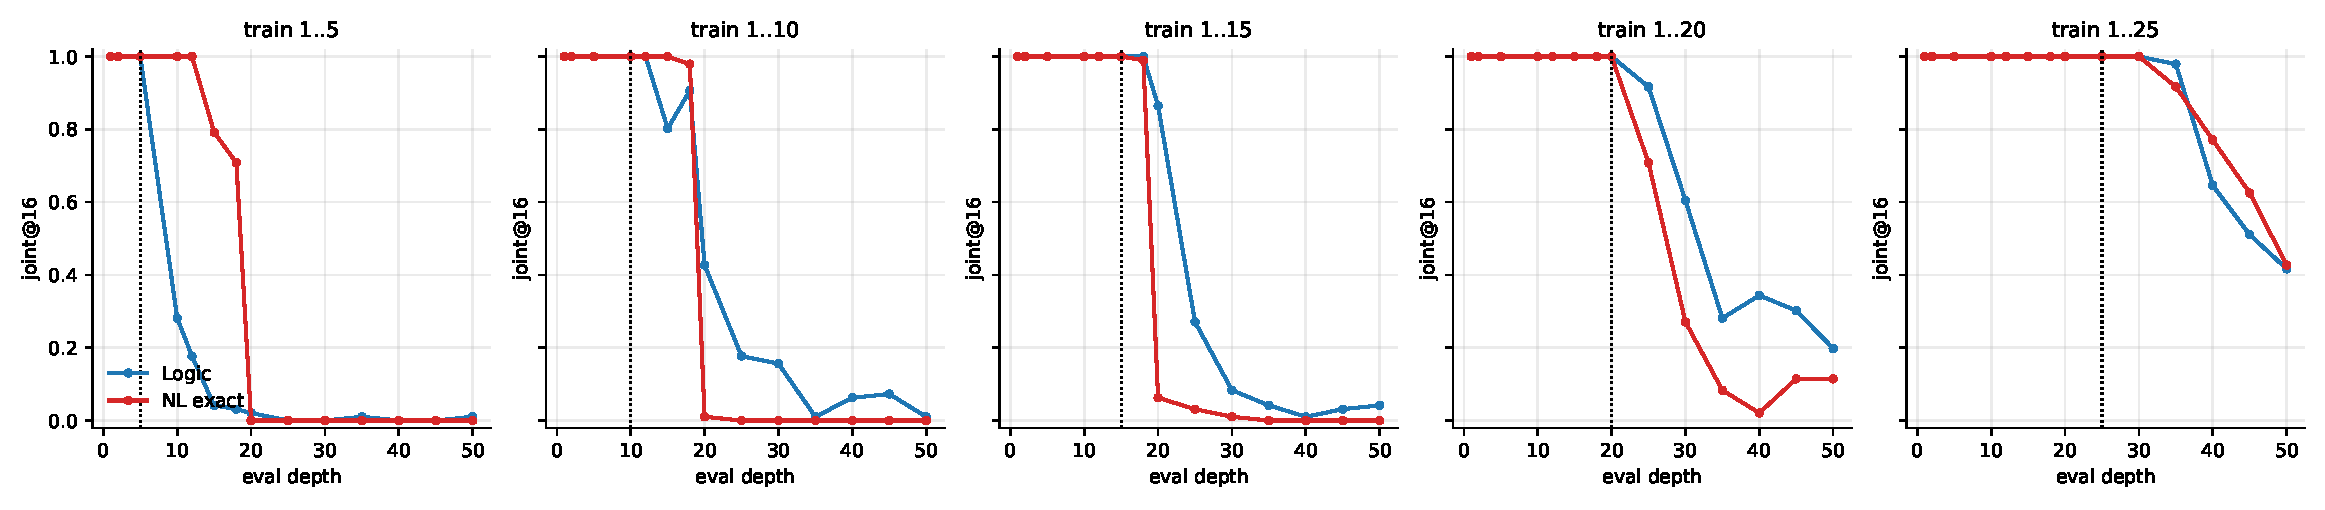
\includegraphics[width=\linewidth]{figures/olmo7b_depth_joint16.pdf}
\caption{Depth curves for final joint correct+valid@16, averaged over seeds.}
\end{figure}
The checkpoint figures below compare each matched logic/NL train-depth pair separately and report only @16.
Main OLMo checkpoint pass@k files available: 100. Full 1k-grid rows now available: logic train1to10 seed3407, logic train1to15 seed3407, logic train1to20 seed3407, logic train1to25 seed3407, logic train1to5 seed3407, NL exact train1to10 seed3407, NL exact train1to15 seed3407, NL exact train1to20 seed3407, NL exact train1to25 seed3407, NL exact train1to5 seed3407.
\begin{figure}[H]\centering
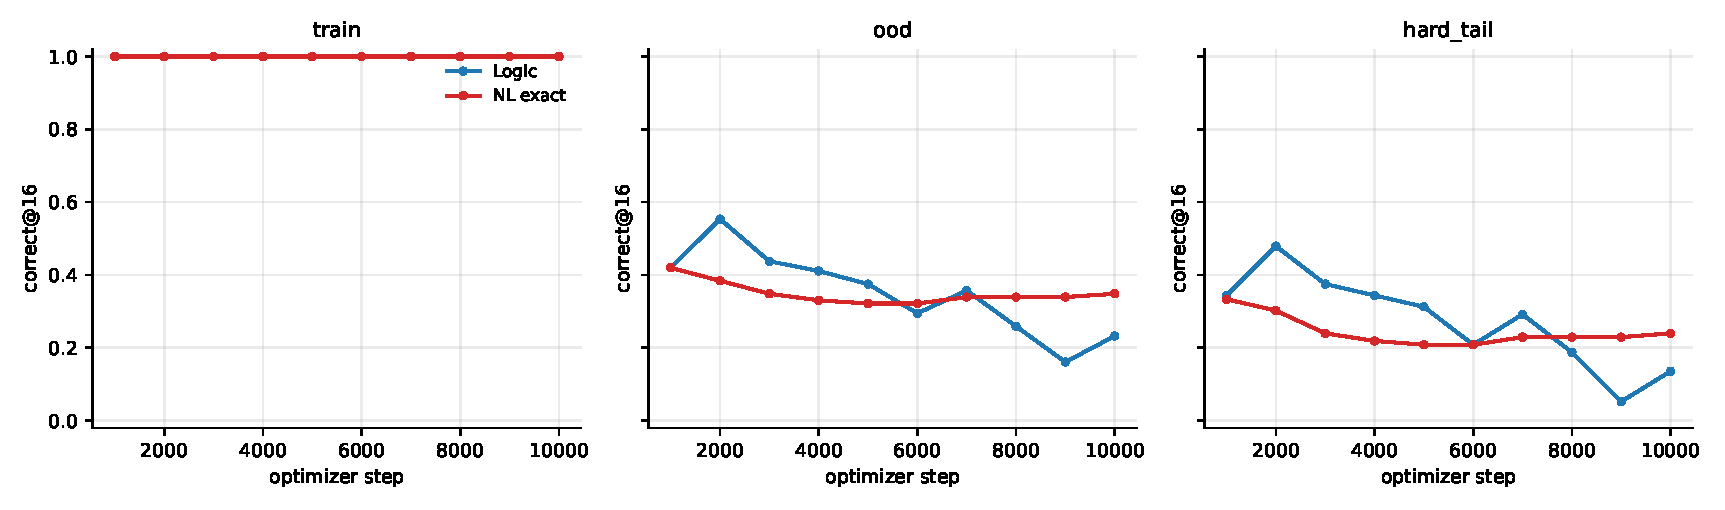
\includegraphics[width=\linewidth]{figures/olmo7b_checkpoint_train1to5_correct16.pdf}
\caption{Seed-3407 train-1-to-5 checkpoint curves for correct@16.}
\end{figure}
\begin{figure}[H]\centering
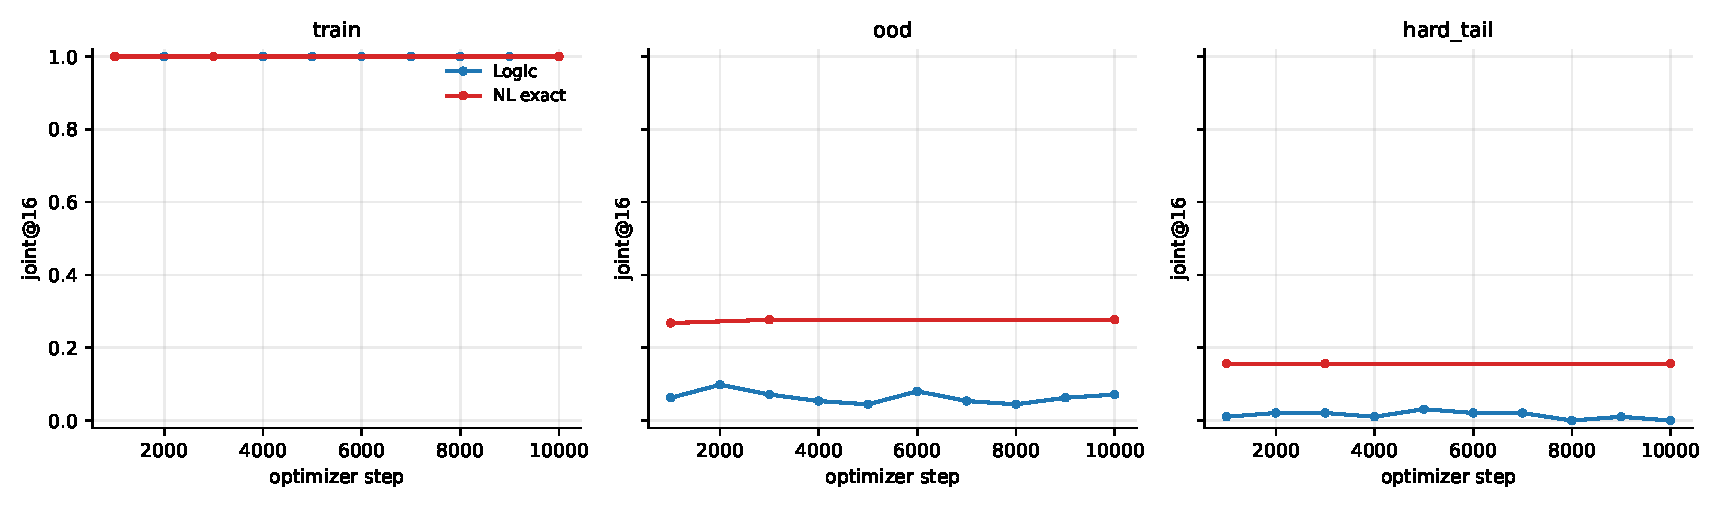
\includegraphics[width=\linewidth]{figures/olmo7b_checkpoint_train1to5_joint16.pdf}
\caption{Seed-3407 train-1-to-5 checkpoint curves for joint correct+valid@16.}
\end{figure}
\begin{figure}[H]\centering
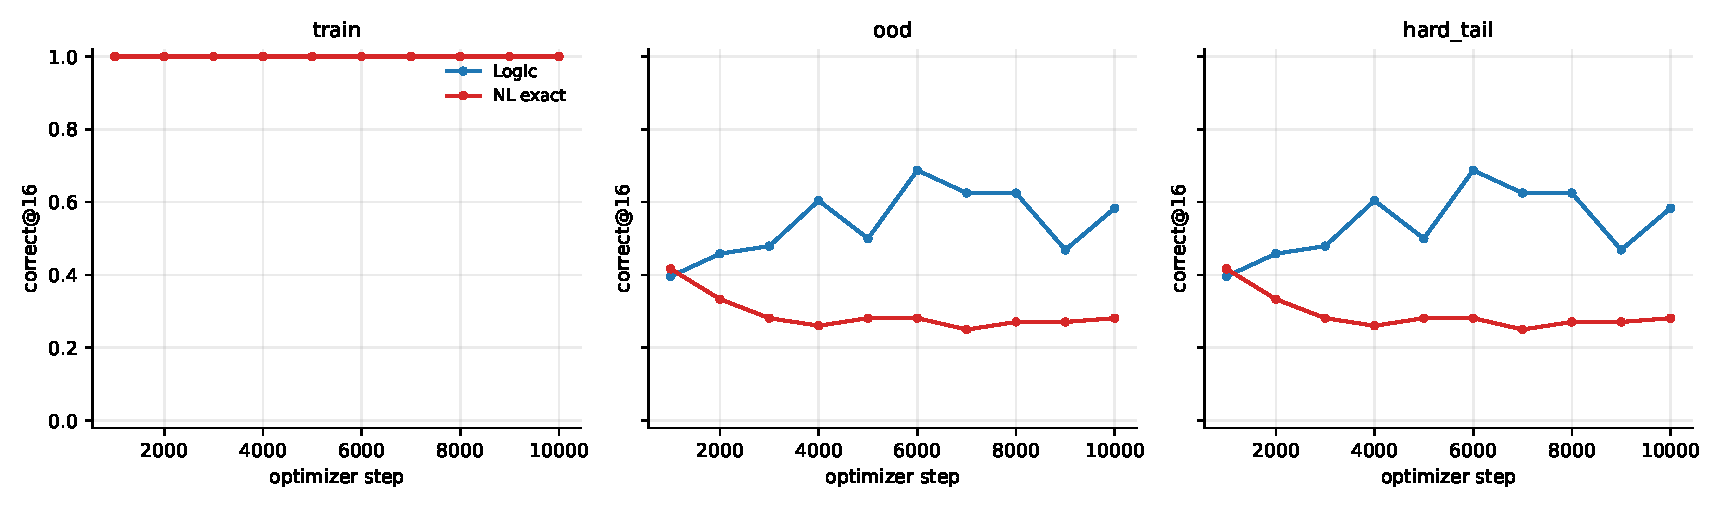
\includegraphics[width=\linewidth]{figures/olmo7b_checkpoint_train1to10_correct16.pdf}
\caption{Seed-3407 train-1-to-10 checkpoint curves for correct@16.}
\end{figure}
\begin{figure}[H]\centering
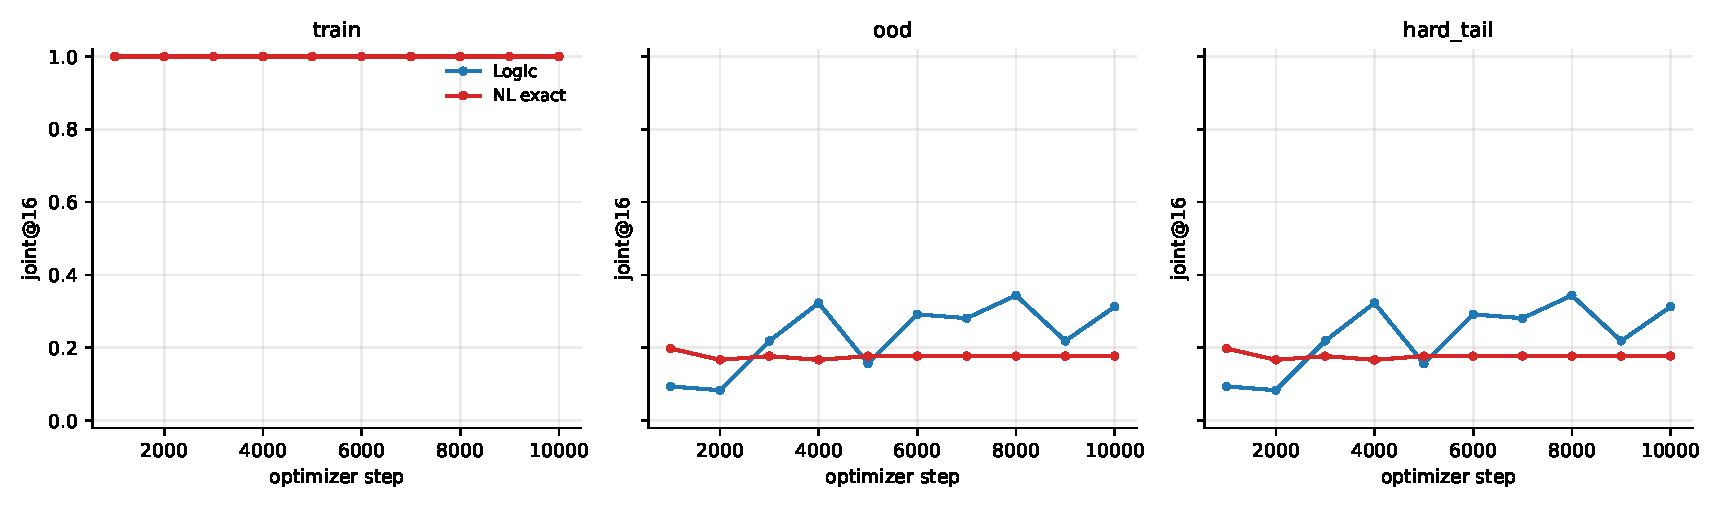
\includegraphics[width=\linewidth]{figures/olmo7b_checkpoint_train1to10_joint16.pdf}
\caption{Seed-3407 train-1-to-10 checkpoint curves for joint correct+valid@16.}
\end{figure}
\begin{figure}[H]\centering
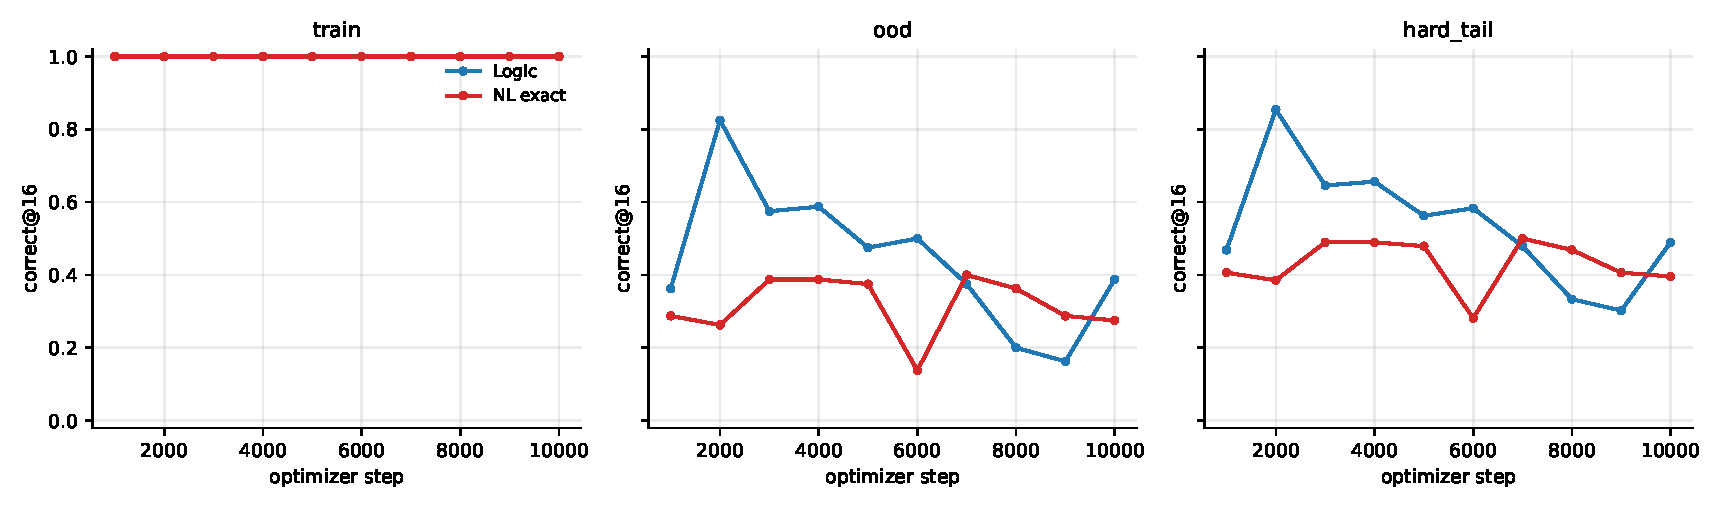
\includegraphics[width=\linewidth]{figures/olmo7b_checkpoint_train1to15_correct16.pdf}
\caption{Seed-3407 train-1-to-15 checkpoint curves for correct@16.}
\end{figure}
\begin{figure}[H]\centering
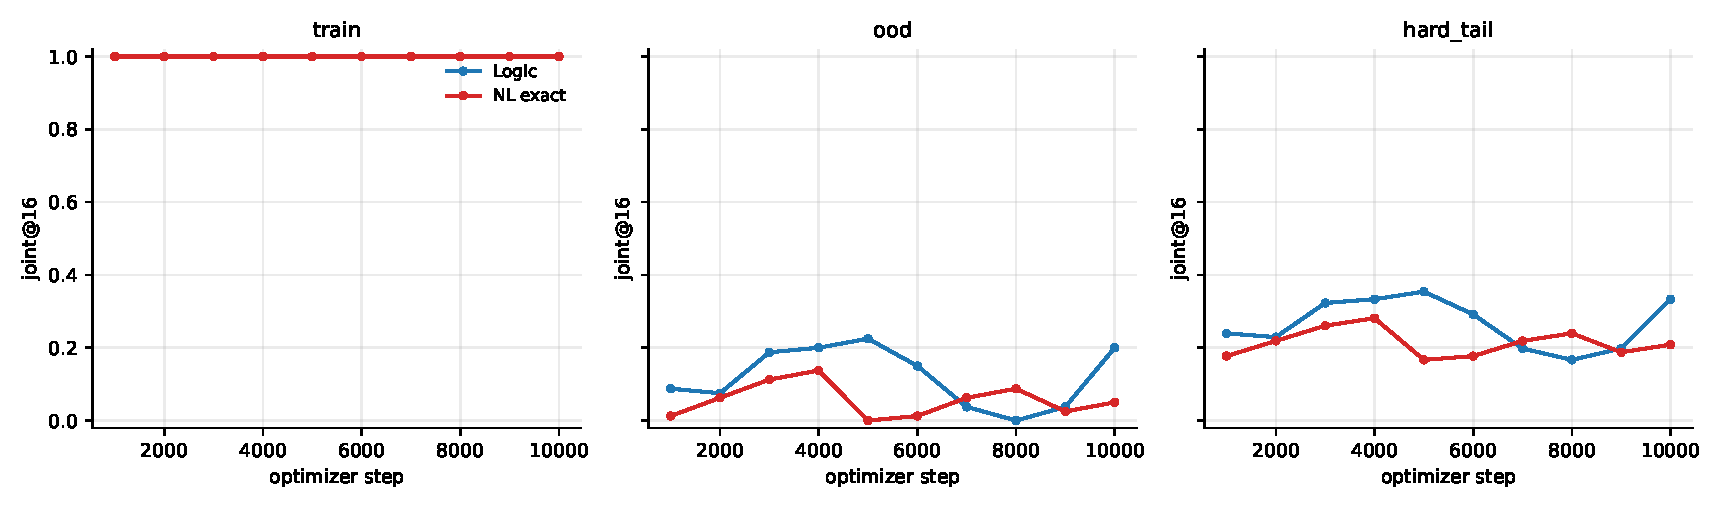
\includegraphics[width=\linewidth]{figures/olmo7b_checkpoint_train1to15_joint16.pdf}
\caption{Seed-3407 train-1-to-15 checkpoint curves for joint correct+valid@16.}
\end{figure}
\begin{figure}[H]\centering
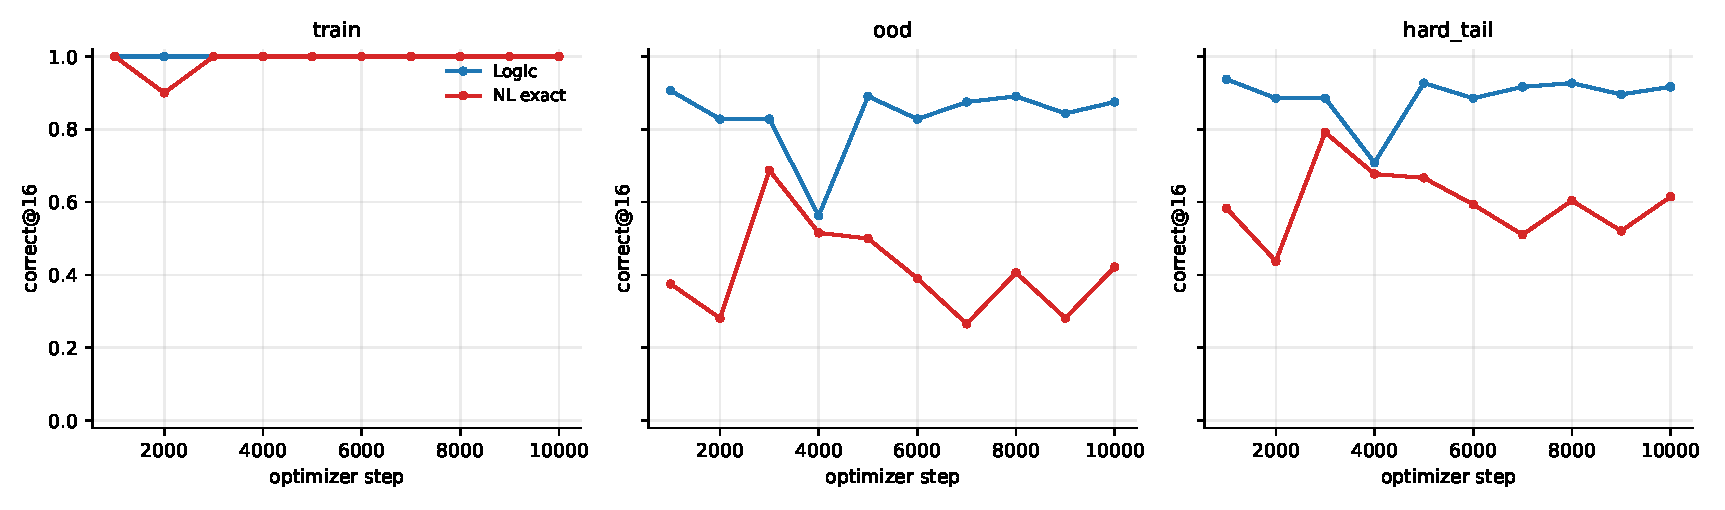
\includegraphics[width=\linewidth]{figures/olmo7b_checkpoint_train1to20_correct16.pdf}
\caption{Seed-3407 train-1-to-20 checkpoint curves for correct@16.}
\end{figure}
\begin{figure}[H]\centering
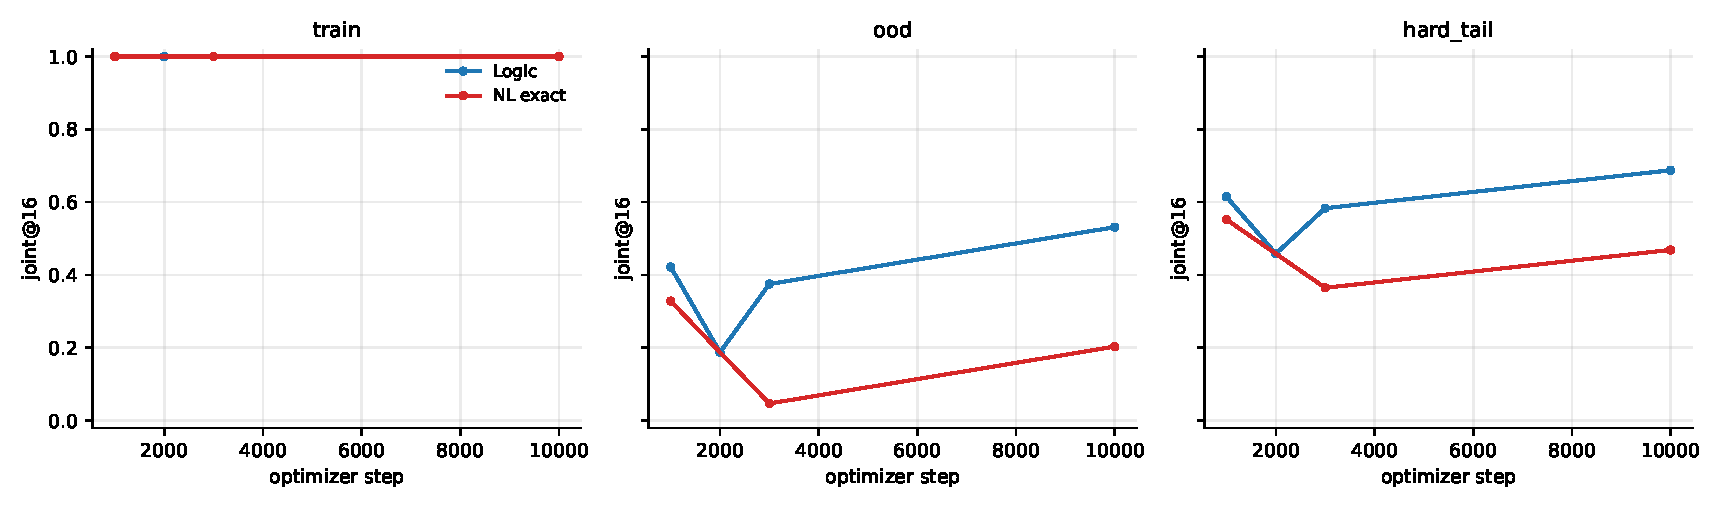
\includegraphics[width=\linewidth]{figures/olmo7b_checkpoint_train1to20_joint16.pdf}
\caption{Seed-3407 train-1-to-20 checkpoint curves for joint correct+valid@16.}
\end{figure}
\begin{figure}[H]\centering
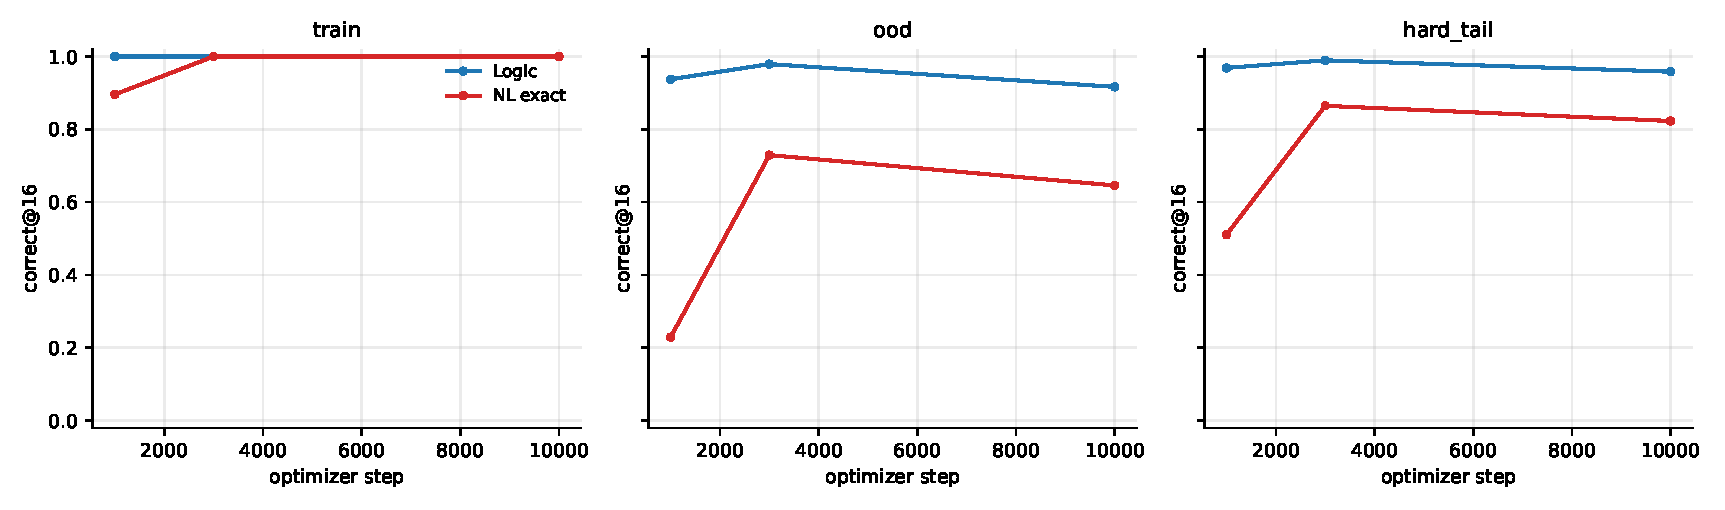
\includegraphics[width=\linewidth]{figures/olmo7b_checkpoint_train1to25_correct16.pdf}
\caption{Seed-3407 train-1-to-25 checkpoint curves for correct@16.}
\end{figure}
\begin{figure}[H]\centering
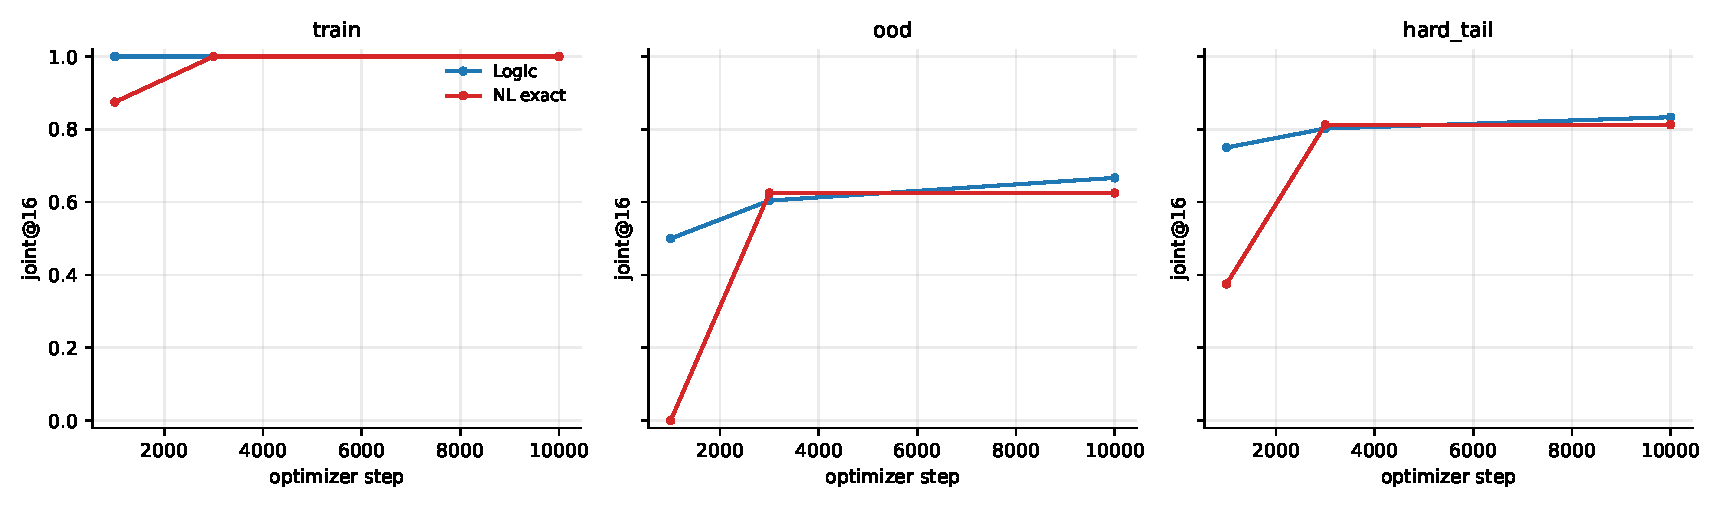
\includegraphics[width=\linewidth]{figures/olmo7b_checkpoint_train1to25_joint16.pdf}
\caption{Seed-3407 train-1-to-25 checkpoint curves for joint correct+valid@16.}
\end{figure}
The next two figures slice the train-1-to-25 checkpoint curve by eval-depth bands. The intermediate protocol contains depths 30, 40, and 50, but not depths 35 or 45, so exact 30--35 or 36--40 curves would require an additional focused checkpoint eval.
\begin{figure}[H]\centering
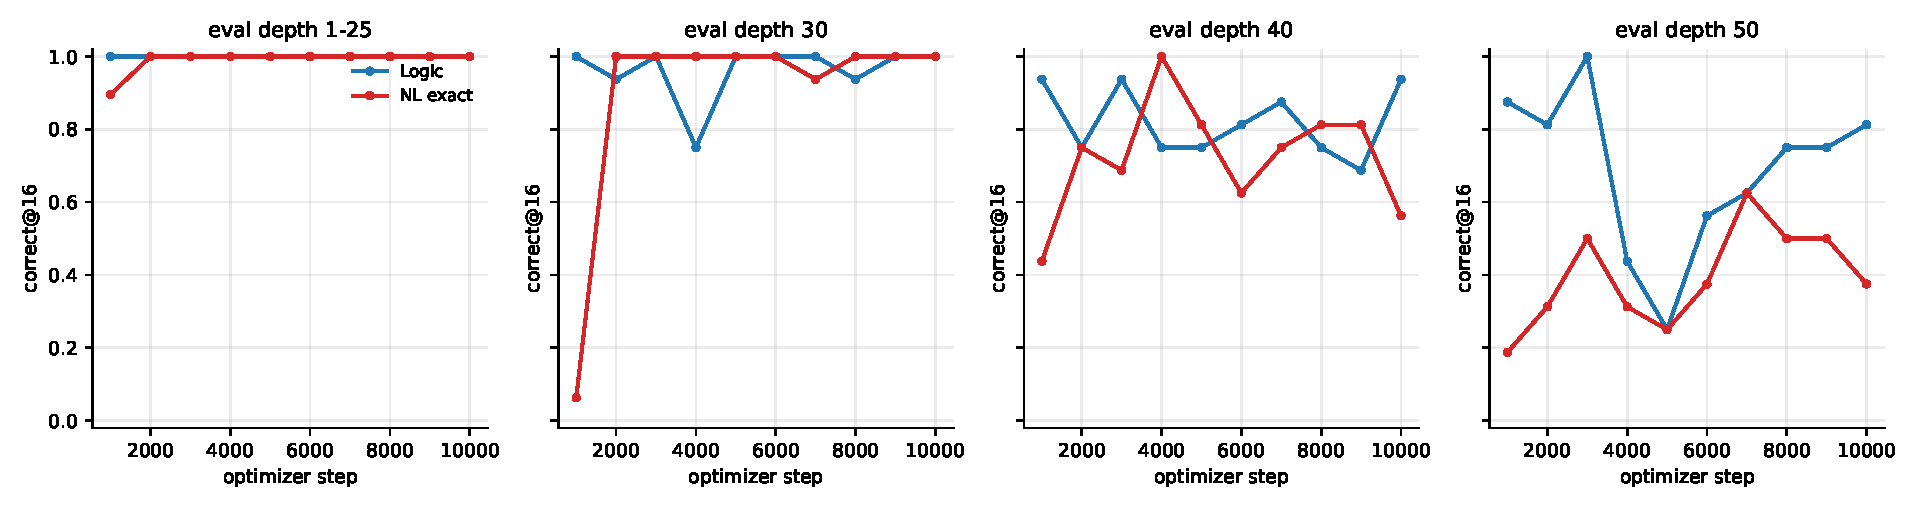
\includegraphics[width=\linewidth]{figures/olmo7b_checkpoint_train1to25_depthbands_correct16.pdf}
\caption{Seed-3407 train-1-to-25 optimizer-step curves for correct@16 over available eval-depth bands.}
\end{figure}
\begin{figure}[H]\centering
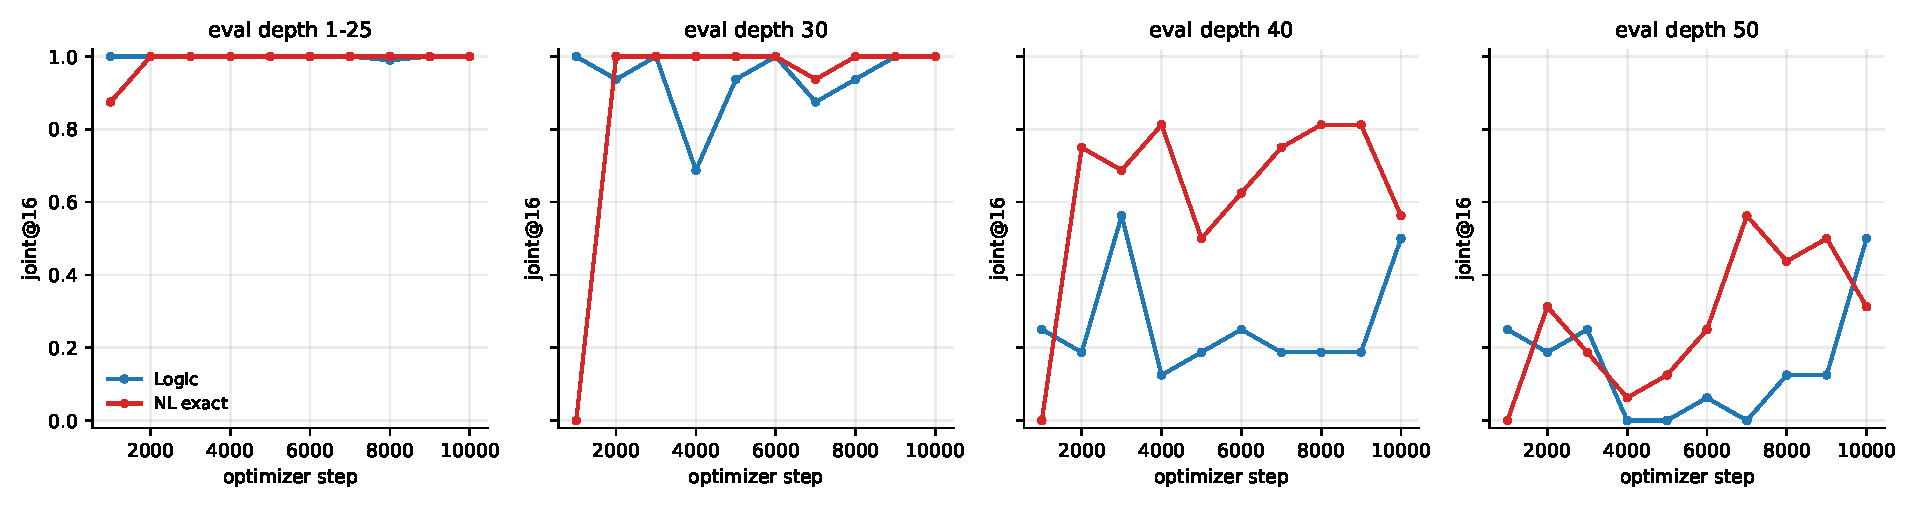
\includegraphics[width=\linewidth]{figures/olmo7b_checkpoint_train1to25_depthbands_joint16.pdf}
\caption{Seed-3407 train-1-to-25 optimizer-step curves for joint correct+valid@16 over available eval-depth bands.}
\end{figure}

\section{Tiny Llama scratch-pretraining result}
These small random-init models were not expected to solve depth-50 extrapolation. The useful signal is that logic is consistently stronger than matched NL on answer-only OOD pass@8, especially at 200M, while strict joint validity remains zero.

\begin{table}[H]
\centering
\small
\begin{tabular}{lllllll}
\toprule
size & template & train c@8 & OOD c@8 & hard c@8 & d50 c@8 & OOD joint@8 \\
\midrule
50m & logic & 0.766 & 0.141 & 0.110 & 0.000 & 0.000 \\
50m & nl\_exact & 0.672 & 0.036 & 0.009 & 0.000 & 0.000 \\
100m & logic & 0.807 & 0.201 & 0.134 & 0.000 & 0.000 \\
100m & nl\_exact & 0.729 & 0.034 & 0.000 & 0.000 & 0.000 \\
200m & logic & 0.854 & 0.240 & 0.146 & 0.000 & 0.000 \\
200m & nl\_exact & 0.719 & 0.047 & 0.018 & 0.000 & 0.000 \\
\bottomrule
\end{tabular}
\caption{Tiny Llama final sparse pass@8 metrics.}
\end{table}

\subsection{Tiny Llama 100k-step rerun}
The 100k-step rerun is complete for all three seeds, sizes, and templates. It does not solve strict depth-50 extrapolation; the notable change is that the 100M NL model improves answer-only OOD correct@8 relative to its 20k run, while joint validity remains zero.

\begin{table}[H]
\centering
\small
\begin{tabular}{llllllll}
\toprule
size & template & train c@8 & OOD c@8 & hard c@8 & d50 c@8 & OOD joint@8 & d50 joint@8 \\
\midrule
50m & logic & 0.807 & 0.112 & 0.074 & 0.000 & 0.000 & 0.000 \\
50m & nl\_exact & 0.630 & 0.068 & 0.060 & 0.000 & 0.000 & 0.000 \\
100m & logic & 0.849 & 0.133 & 0.077 & 0.000 & 0.000 & 0.000 \\
100m & nl\_exact & 0.672 & 0.258 & 0.199 & 0.021 & 0.000 & 0.000 \\
200m & logic & 0.625 & 0.201 & 0.134 & 0.000 & 0.008 & 0.000 \\
200m & nl\_exact & 0.583 & 0.055 & 0.033 & 0.000 & 0.000 & 0.000 \\
\bottomrule
\end{tabular}
\caption{Tiny Llama 100k-step final sparse pass@8 metrics.}
\end{table}

Tiny 100k checkpoint pass@k rows available at report generation time: 90; the completed grid contains checkpoints 20k, 40k, 60k, 80k, and 100k for every size/template/seed.
\begin{figure}[H]\centering
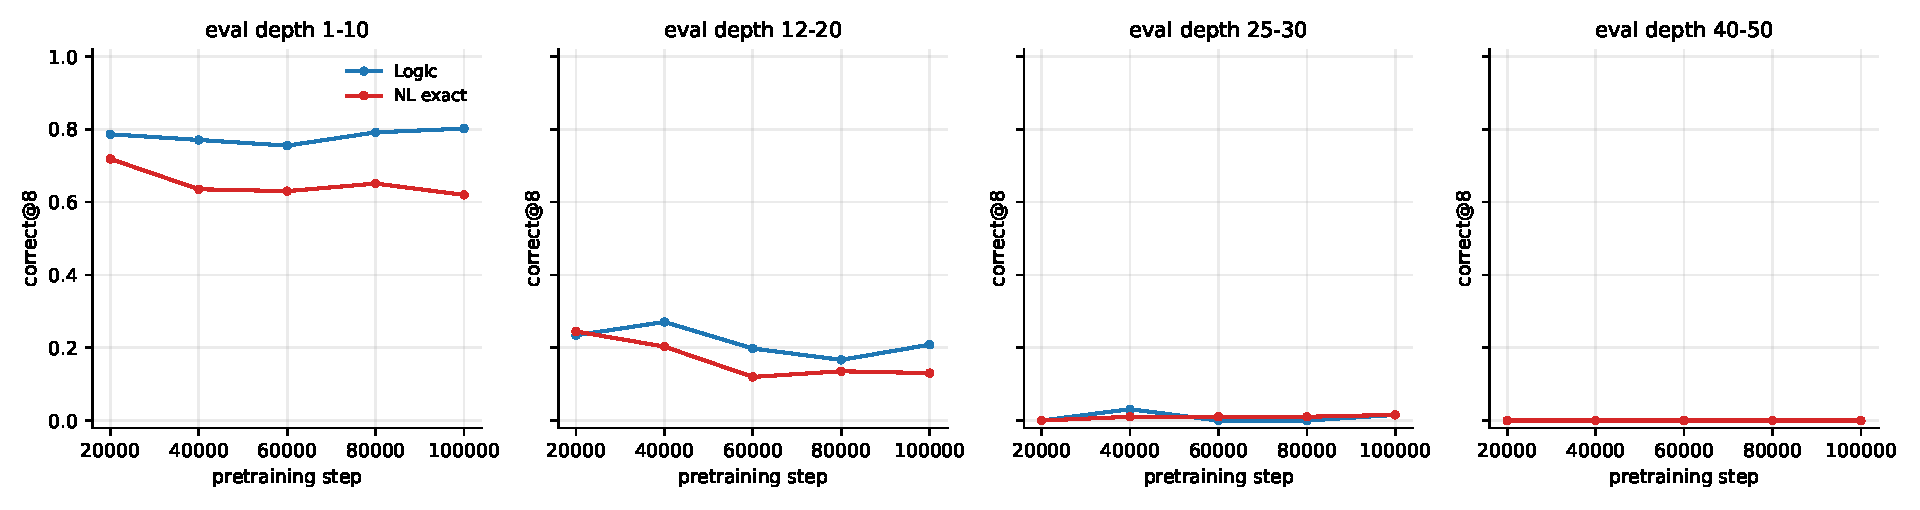
\includegraphics[width=\linewidth]{figures/tiny_llama_100k_50m_checkpoint_depthbands_correct_k8.pdf}
\caption{Tiny Llama 100k 50m optimizer-step curves for correct@8 over eval-depth bands.}
\end{figure}
\begin{figure}[H]\centering
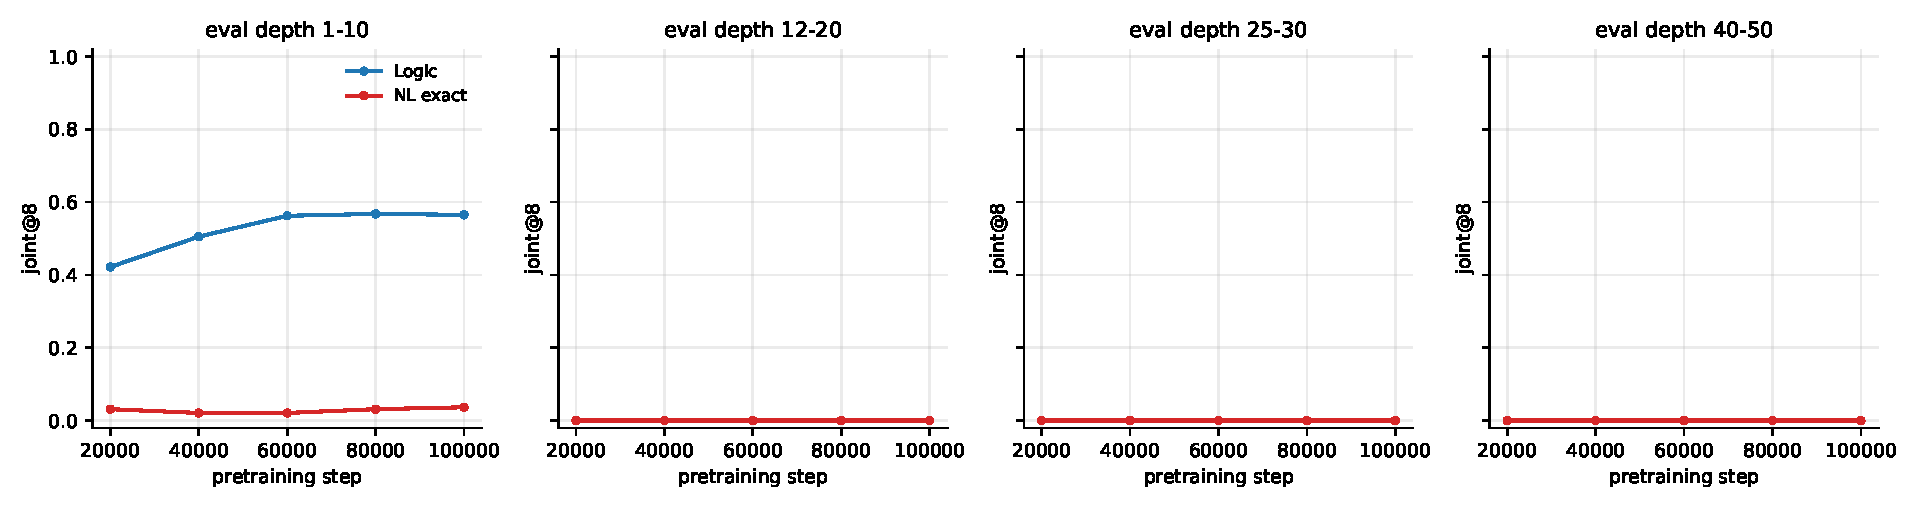
\includegraphics[width=\linewidth]{figures/tiny_llama_100k_50m_checkpoint_depthbands_joint_k8.pdf}
\caption{Tiny Llama 100k 50m optimizer-step curves for joint correct+valid@8 over eval-depth bands.}
\end{figure}
\begin{figure}[H]\centering
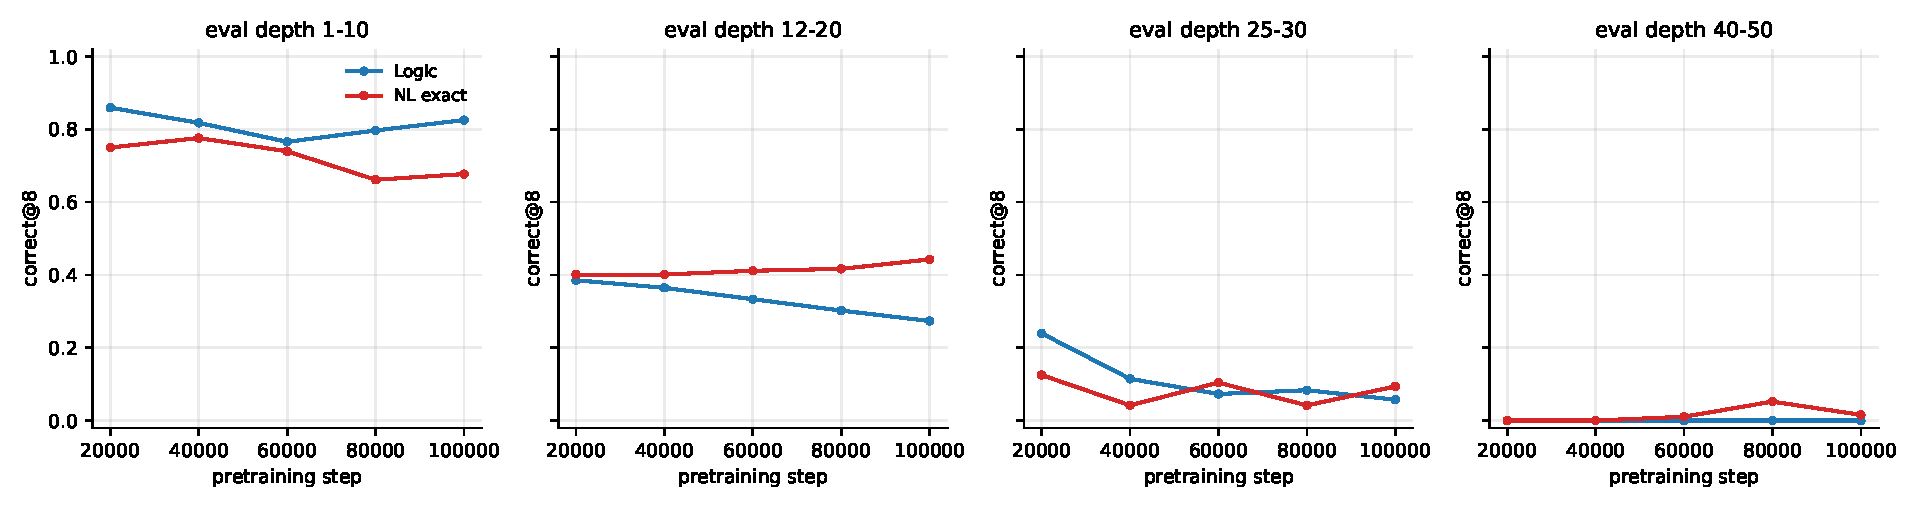
\includegraphics[width=\linewidth]{figures/tiny_llama_100k_100m_checkpoint_depthbands_correct_k8.pdf}
\caption{Tiny Llama 100k 100m optimizer-step curves for correct@8 over eval-depth bands.}
\end{figure}
\begin{figure}[H]\centering
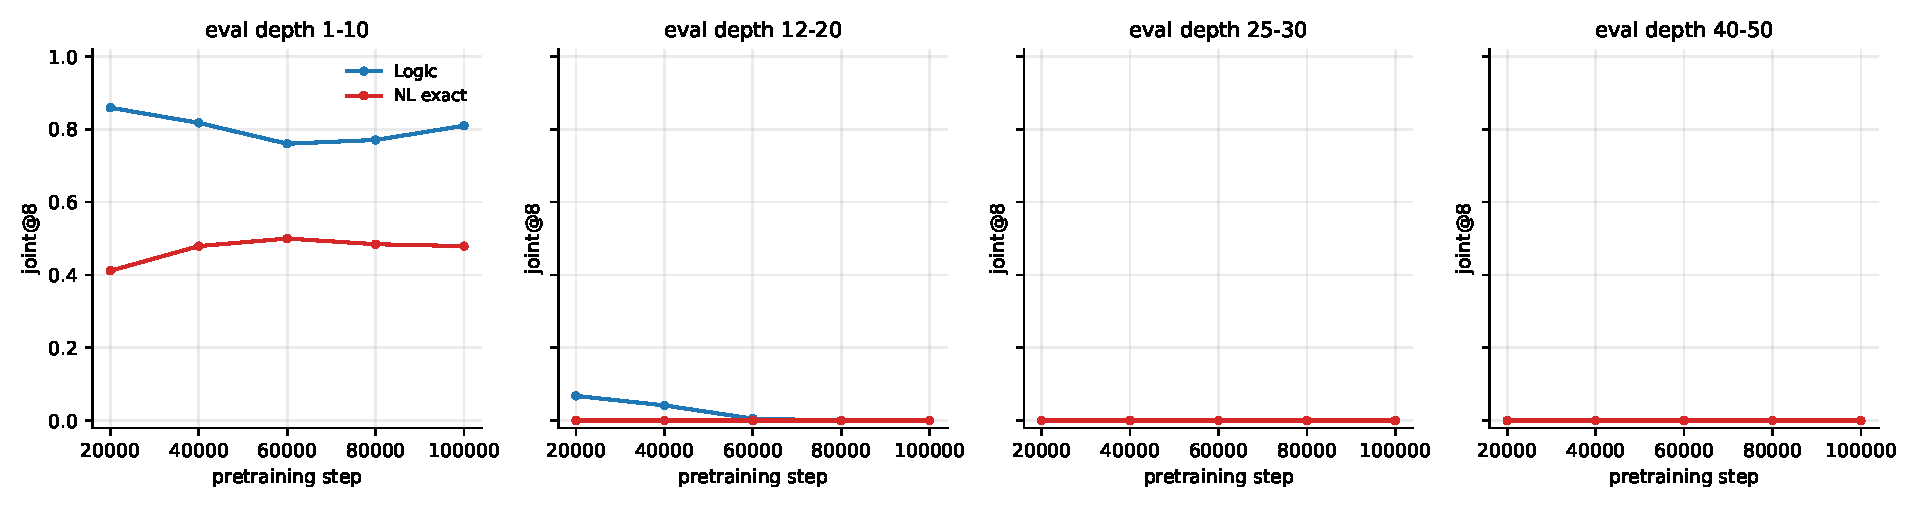
\includegraphics[width=\linewidth]{figures/tiny_llama_100k_100m_checkpoint_depthbands_joint_k8.pdf}
\caption{Tiny Llama 100k 100m optimizer-step curves for joint correct+valid@8 over eval-depth bands.}
\end{figure}
\begin{figure}[H]\centering
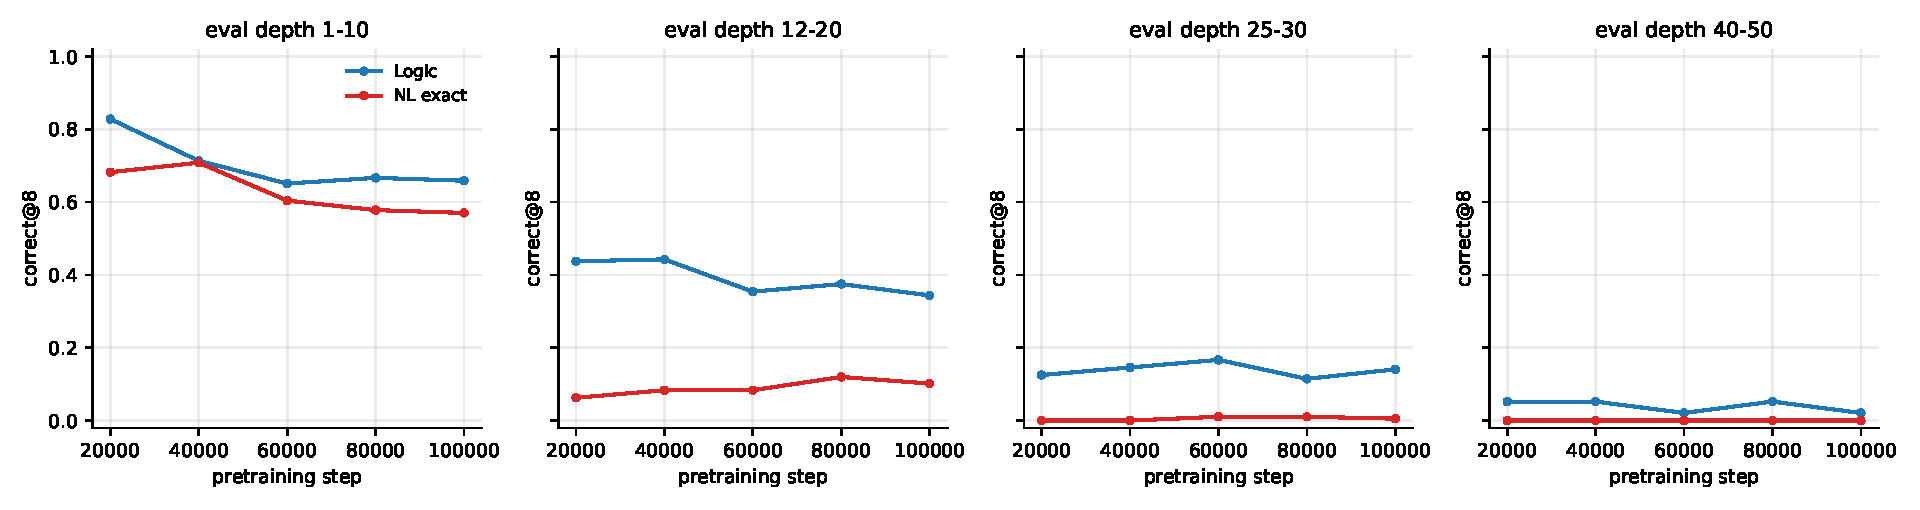
\includegraphics[width=\linewidth]{figures/tiny_llama_100k_200m_checkpoint_depthbands_correct_k8.pdf}
\caption{Tiny Llama 100k 200m optimizer-step curves for correct@8 over eval-depth bands.}
\end{figure}
\begin{figure}[H]\centering
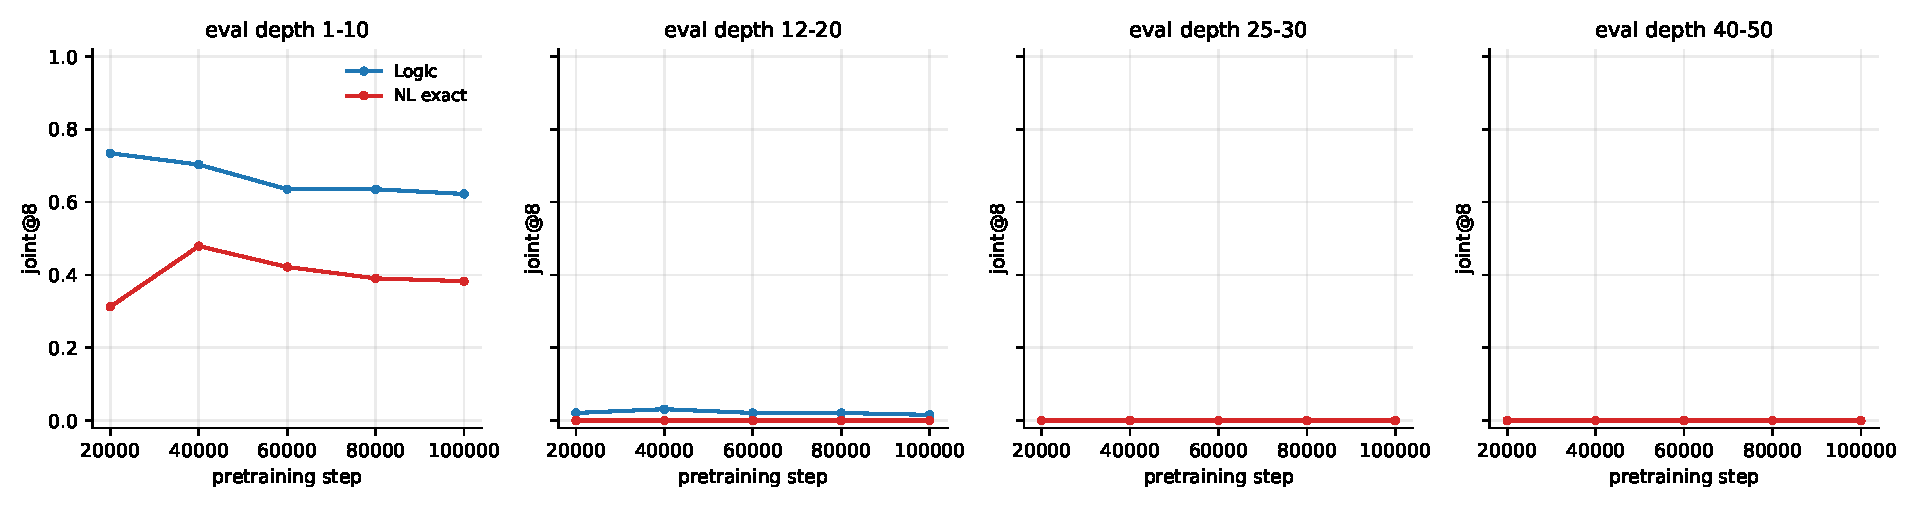
\includegraphics[width=\linewidth]{figures/tiny_llama_100k_200m_checkpoint_depthbands_joint_k8.pdf}
\caption{Tiny Llama 100k 200m optimizer-step curves for joint correct+valid@8 over eval-depth bands.}
\end{figure}

The tiny plots separate model sizes and separate answer correctness from joint correct+valid.
\begin{figure}[H]\centering
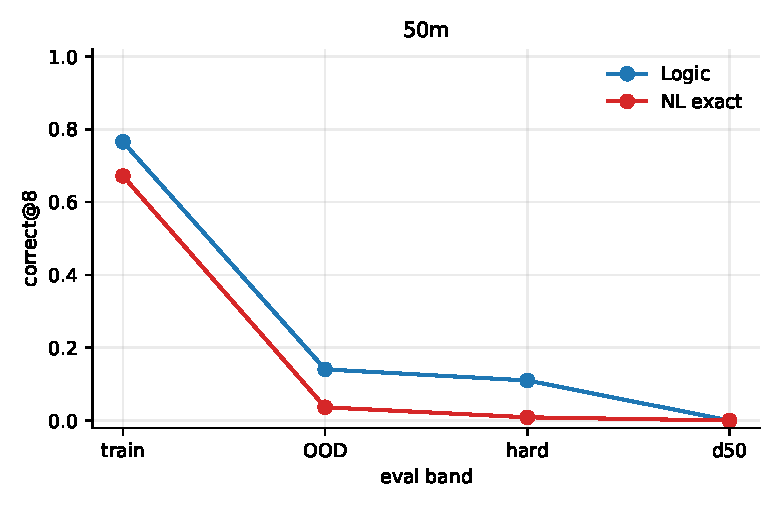
\includegraphics[width=0.72\linewidth]{figures/tiny_llama_50m_bands_correct_k8.pdf}
\caption{Tiny Llama 50m train/OOD/hard-tail/depth-50 correct@8 by template.}
\end{figure}
\begin{figure}[H]\centering
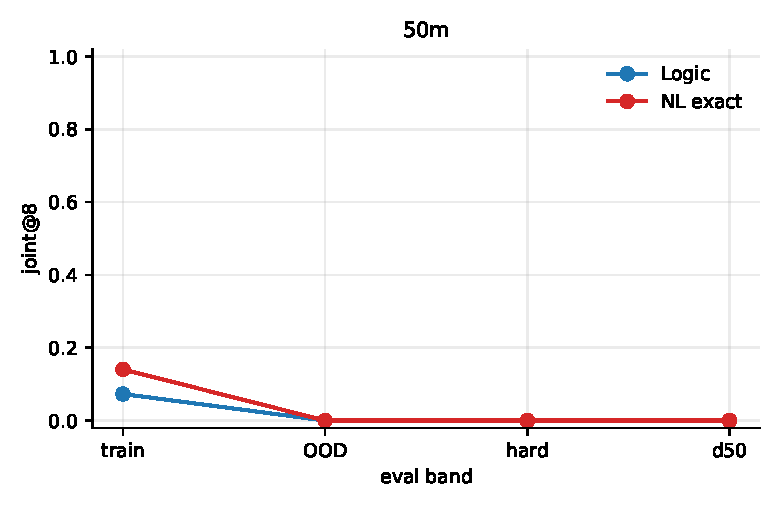
\includegraphics[width=0.72\linewidth]{figures/tiny_llama_50m_bands_joint_k8.pdf}
\caption{Tiny Llama 50m train/OOD/hard-tail/depth-50 joint correct+valid@8 by template.}
\end{figure}
\begin{figure}[H]\centering
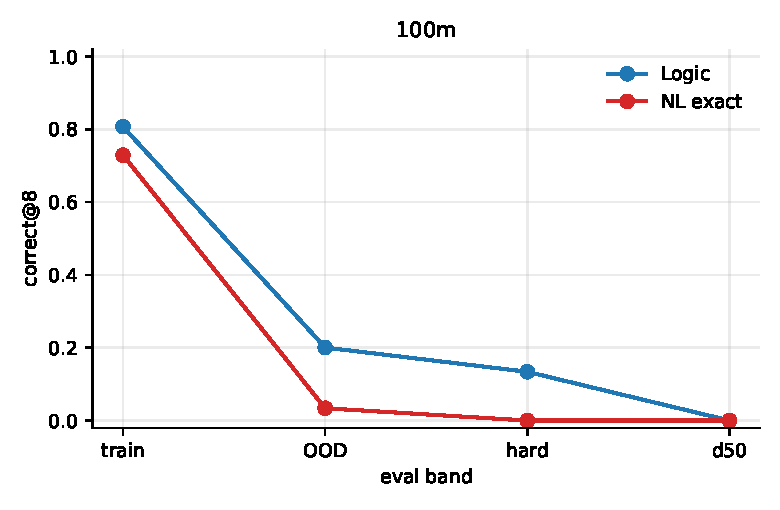
\includegraphics[width=0.72\linewidth]{figures/tiny_llama_100m_bands_correct_k8.pdf}
\caption{Tiny Llama 100m train/OOD/hard-tail/depth-50 correct@8 by template.}
\end{figure}
\begin{figure}[H]\centering
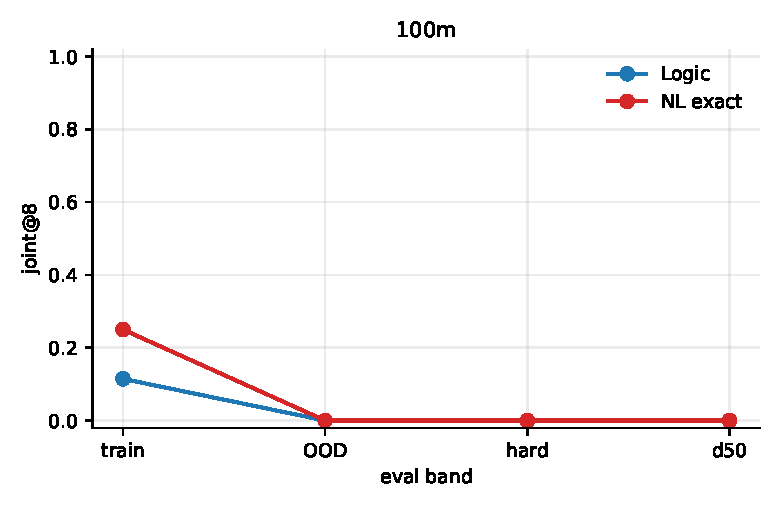
\includegraphics[width=0.72\linewidth]{figures/tiny_llama_100m_bands_joint_k8.pdf}
\caption{Tiny Llama 100m train/OOD/hard-tail/depth-50 joint correct+valid@8 by template.}
\end{figure}
\begin{figure}[H]\centering
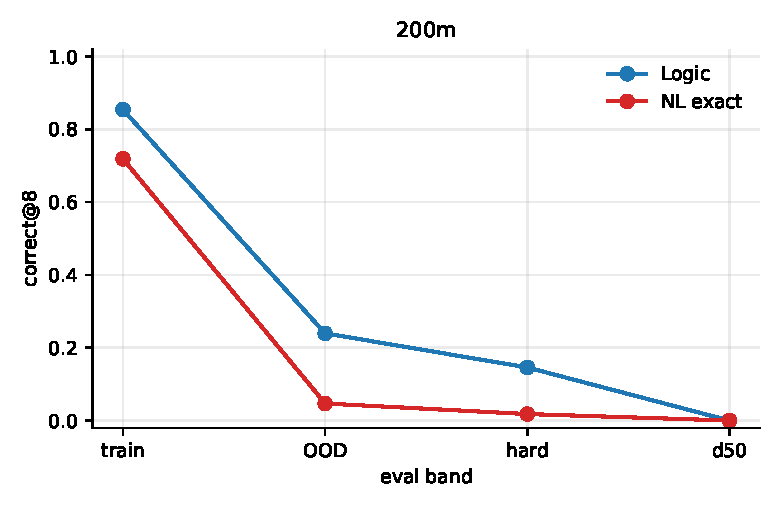
\includegraphics[width=0.72\linewidth]{figures/tiny_llama_200m_bands_correct_k8.pdf}
\caption{Tiny Llama 200m train/OOD/hard-tail/depth-50 correct@8 by template.}
\end{figure}
\begin{figure}[H]\centering
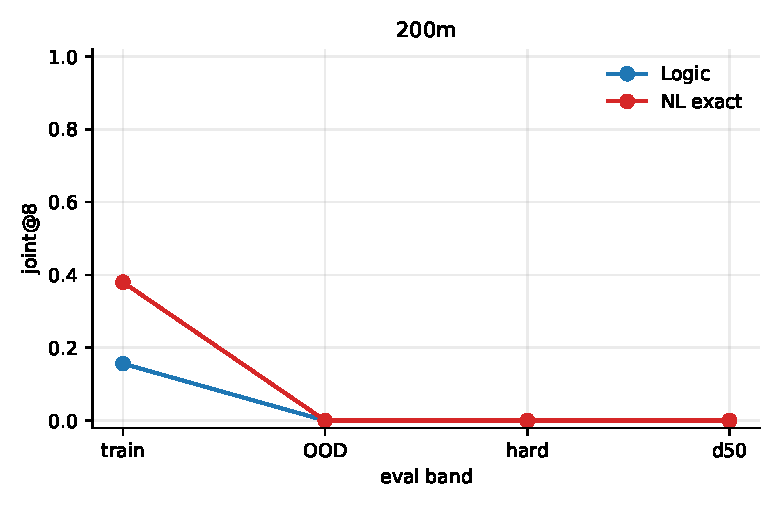
\includegraphics[width=0.72\linewidth]{figures/tiny_llama_200m_bands_joint_k8.pdf}
\caption{Tiny Llama 200m train/OOD/hard-tail/depth-50 joint correct+valid@8 by template.}
\end{figure}
\begin{figure}[H]\centering
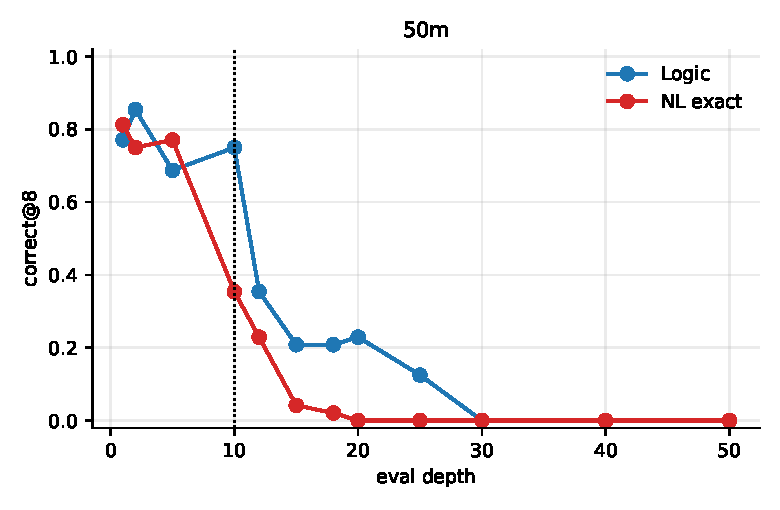
\includegraphics[width=0.72\linewidth]{figures/tiny_llama_50m_depth_correct_k8.pdf}
\caption{Tiny Llama 50m seed-mean depth curve for correct@8. The dotted line marks train max depth 10.}
\end{figure}
\begin{figure}[H]\centering
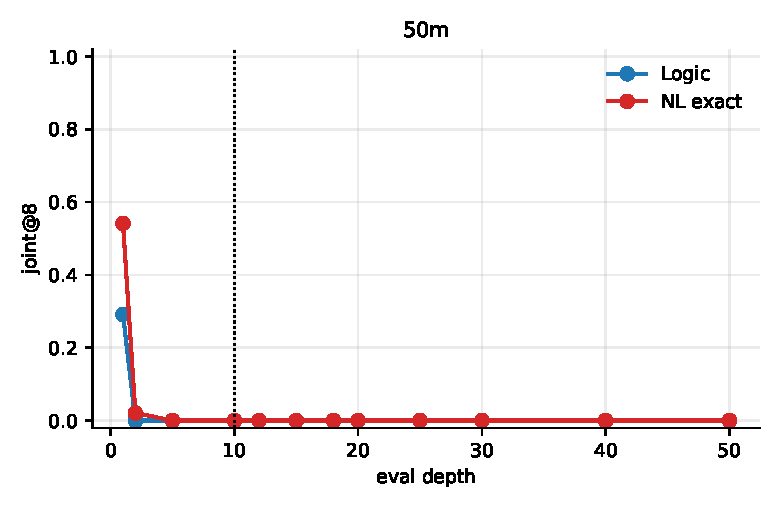
\includegraphics[width=0.72\linewidth]{figures/tiny_llama_50m_depth_joint_k8.pdf}
\caption{Tiny Llama 50m seed-mean depth curve for joint correct+valid@8. The dotted line marks train max depth 10.}
\end{figure}
\begin{figure}[H]\centering
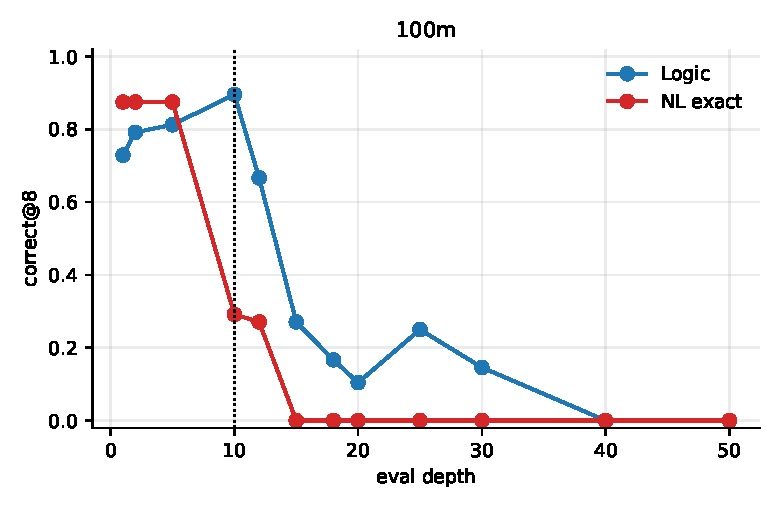
\includegraphics[width=0.72\linewidth]{figures/tiny_llama_100m_depth_correct_k8.pdf}
\caption{Tiny Llama 100m seed-mean depth curve for correct@8. The dotted line marks train max depth 10.}
\end{figure}
\begin{figure}[H]\centering
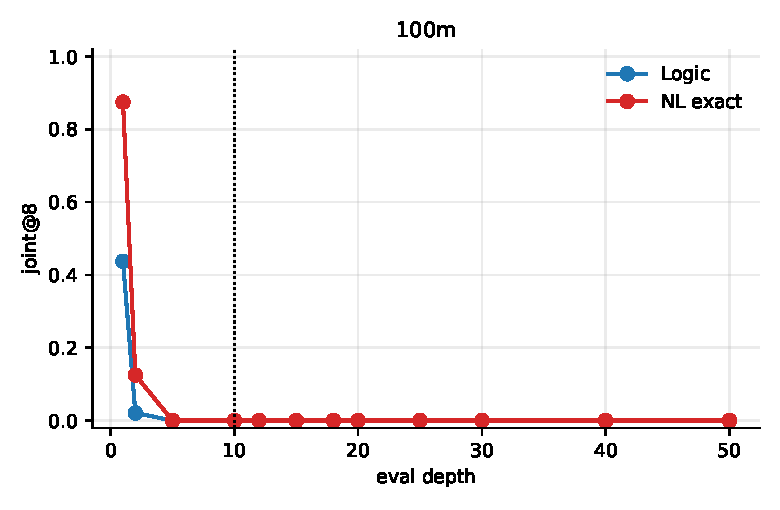
\includegraphics[width=0.72\linewidth]{figures/tiny_llama_100m_depth_joint_k8.pdf}
\caption{Tiny Llama 100m seed-mean depth curve for joint correct+valid@8. The dotted line marks train max depth 10.}
\end{figure}
\begin{figure}[H]\centering
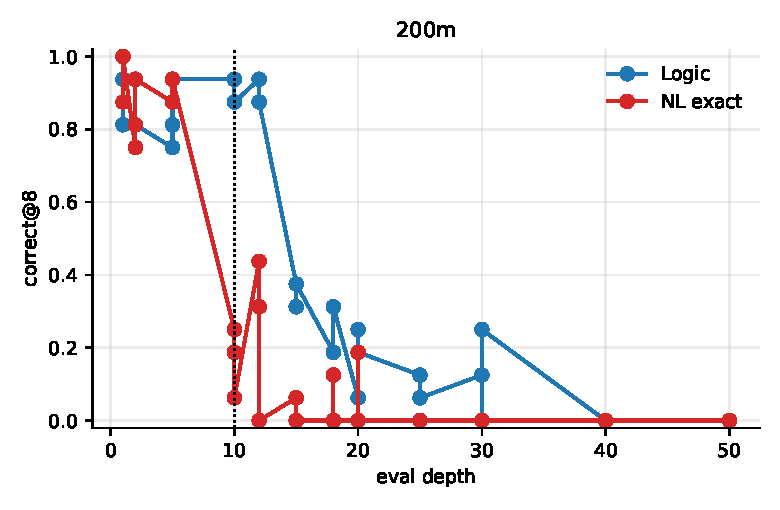
\includegraphics[width=0.72\linewidth]{figures/tiny_llama_200m_depth_correct_k8.pdf}
\caption{Tiny Llama 200m seed-mean depth curve for correct@8. The dotted line marks train max depth 10.}
\end{figure}
\begin{figure}[H]\centering
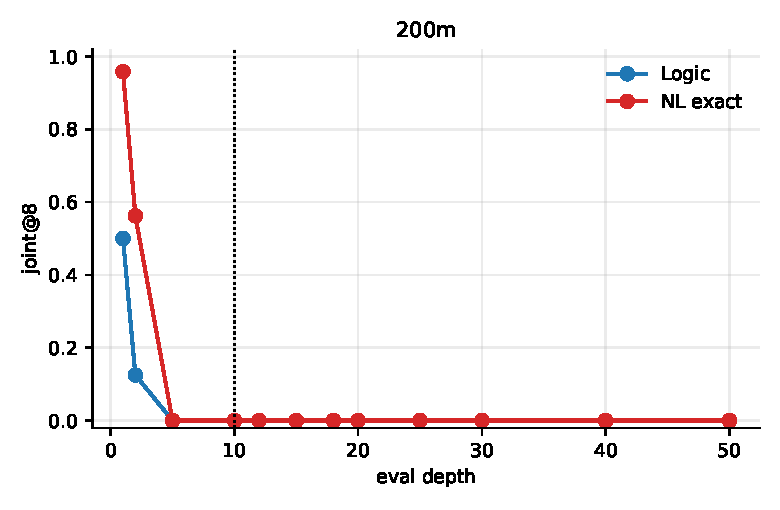
\includegraphics[width=0.72\linewidth]{figures/tiny_llama_200m_depth_joint_k8.pdf}
\caption{Tiny Llama 200m seed-mean depth curve for joint correct+valid@8. The dotted line marks train max depth 10.}
\end{figure}

Tiny checkpoint pass@k rows available at report generation time: 36. The curves below include all available intermediate checkpoint rows plus the final 20k checkpoint.

\begin{figure}[H]\centering
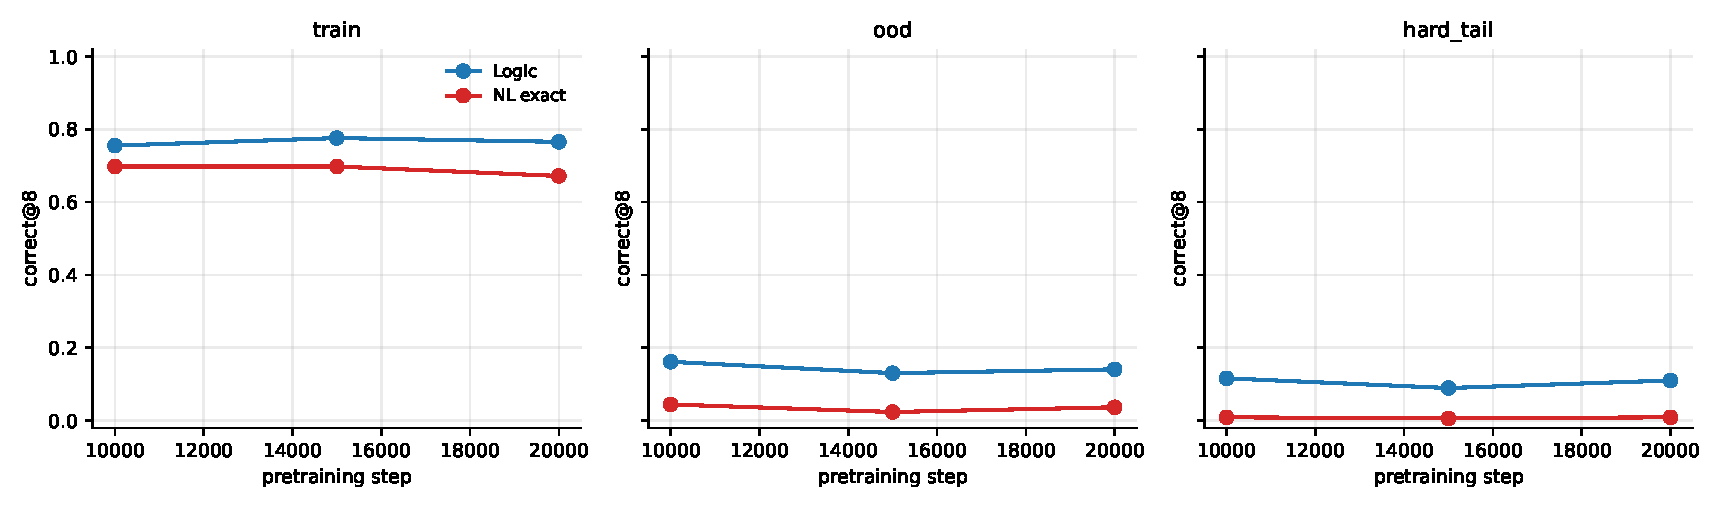
\includegraphics[width=\linewidth]{figures/tiny_llama_50m_checkpoint_correct_k8.pdf}
\caption{Tiny Llama 50m seed-mean checkpoint curves for correct@8.}
\end{figure}
\begin{figure}[H]\centering
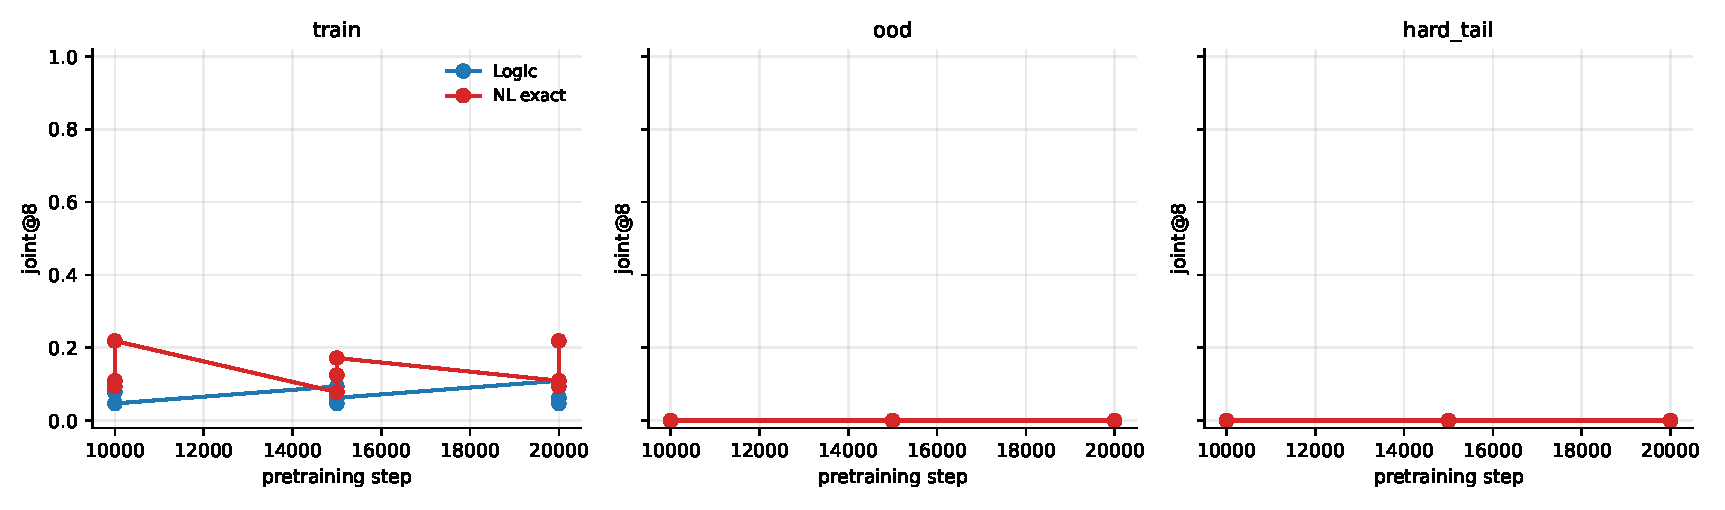
\includegraphics[width=\linewidth]{figures/tiny_llama_50m_checkpoint_joint_k8.pdf}
\caption{Tiny Llama 50m seed-mean checkpoint curves for joint correct+valid@8.}
\end{figure}
\begin{figure}[H]\centering
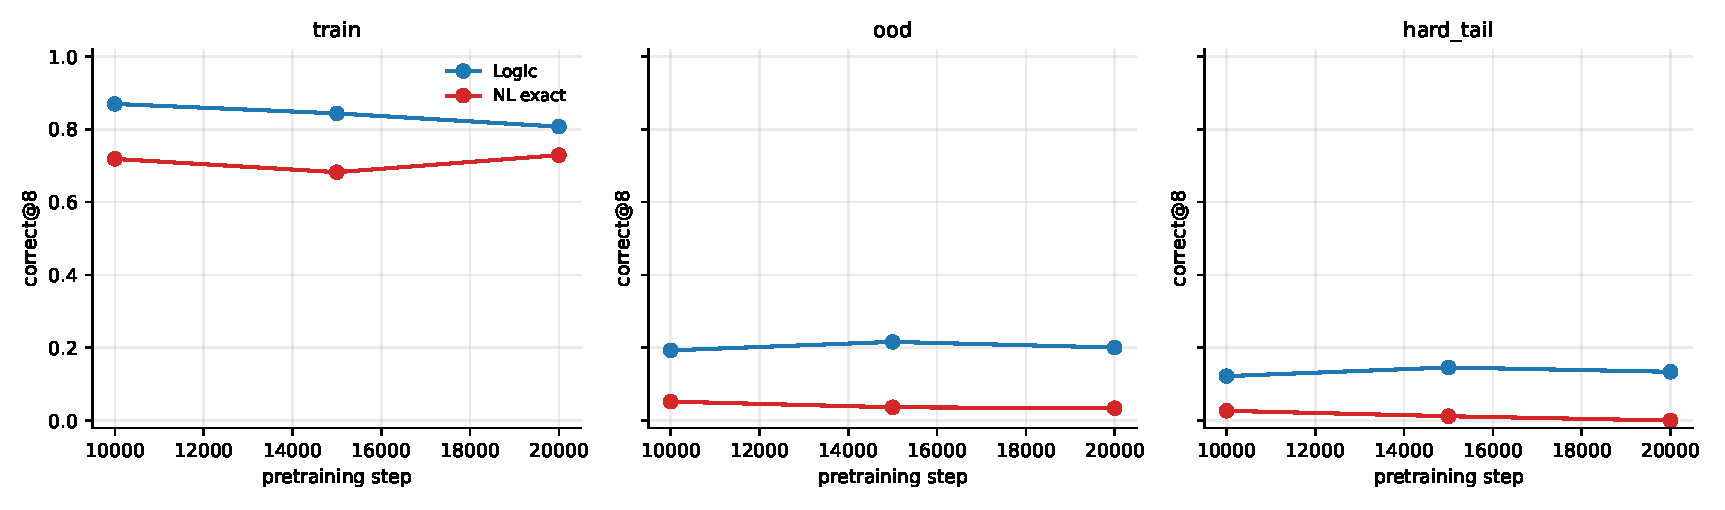
\includegraphics[width=\linewidth]{figures/tiny_llama_100m_checkpoint_correct_k8.pdf}
\caption{Tiny Llama 100m seed-mean checkpoint curves for correct@8.}
\end{figure}
\begin{figure}[H]\centering
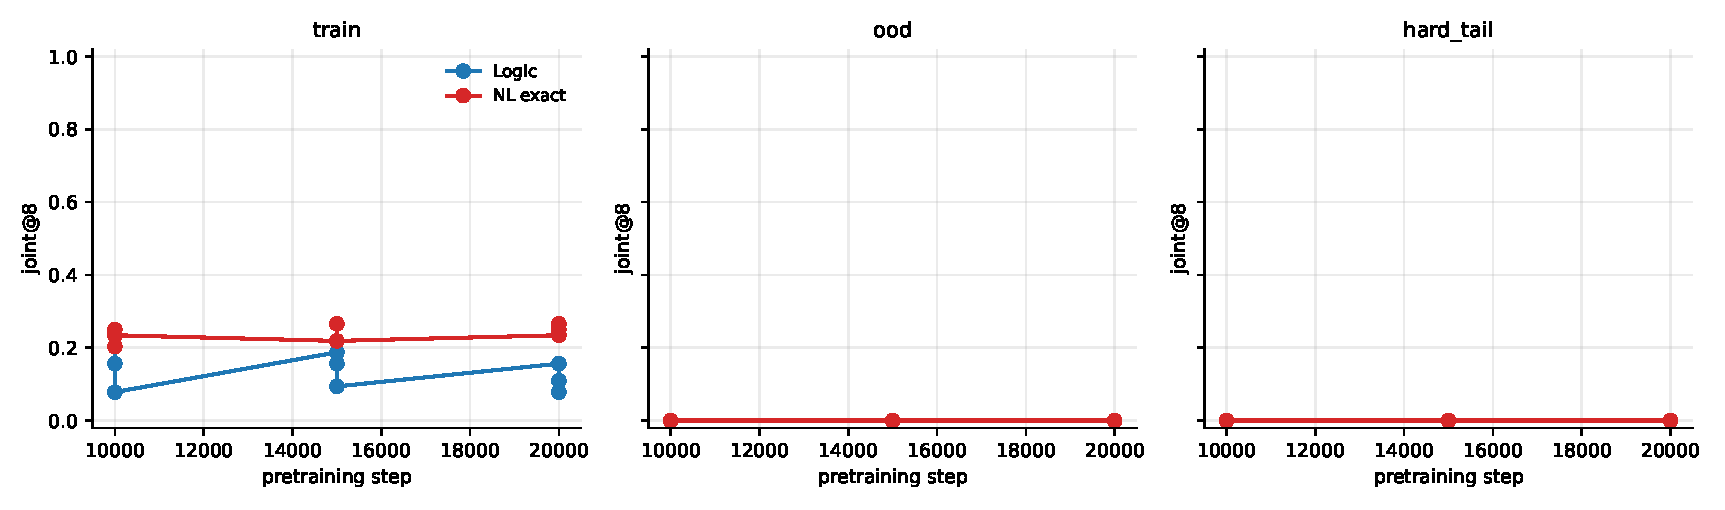
\includegraphics[width=\linewidth]{figures/tiny_llama_100m_checkpoint_joint_k8.pdf}
\caption{Tiny Llama 100m seed-mean checkpoint curves for joint correct+valid@8.}
\end{figure}
\begin{figure}[H]\centering
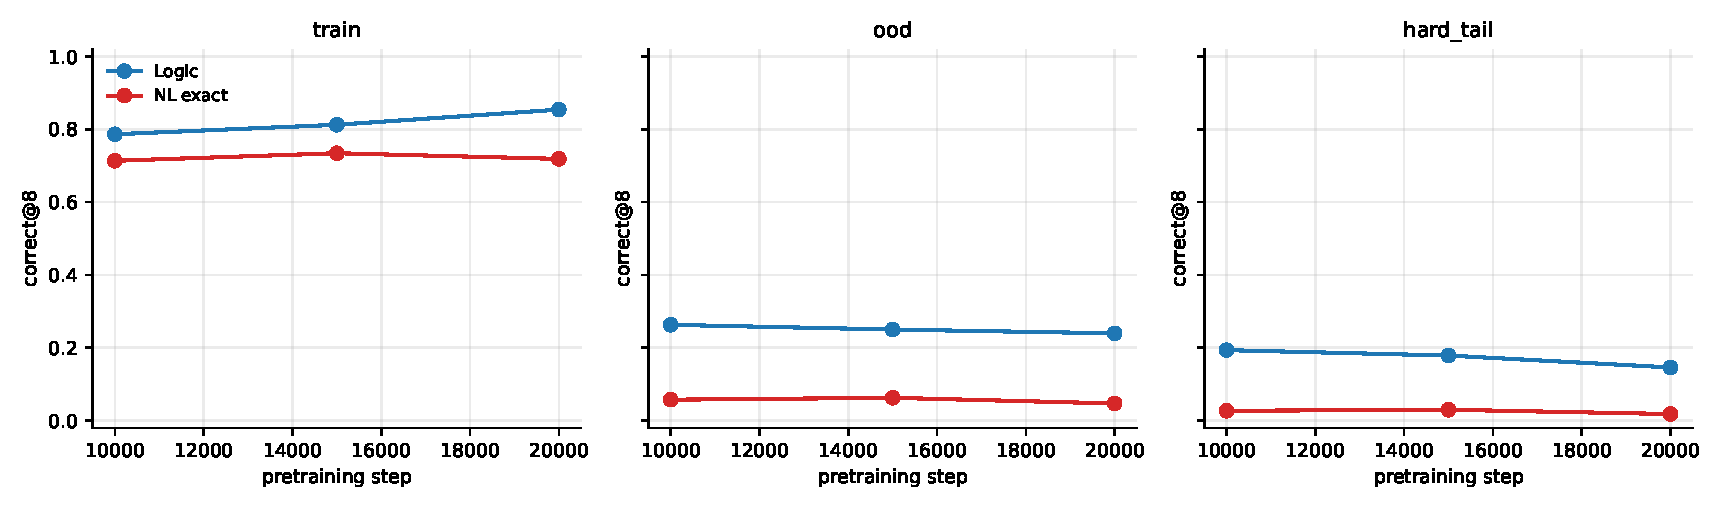
\includegraphics[width=\linewidth]{figures/tiny_llama_200m_checkpoint_correct_k8.pdf}
\caption{Tiny Llama 200m seed-mean checkpoint curves for correct@8.}
\end{figure}
\begin{figure}[H]\centering
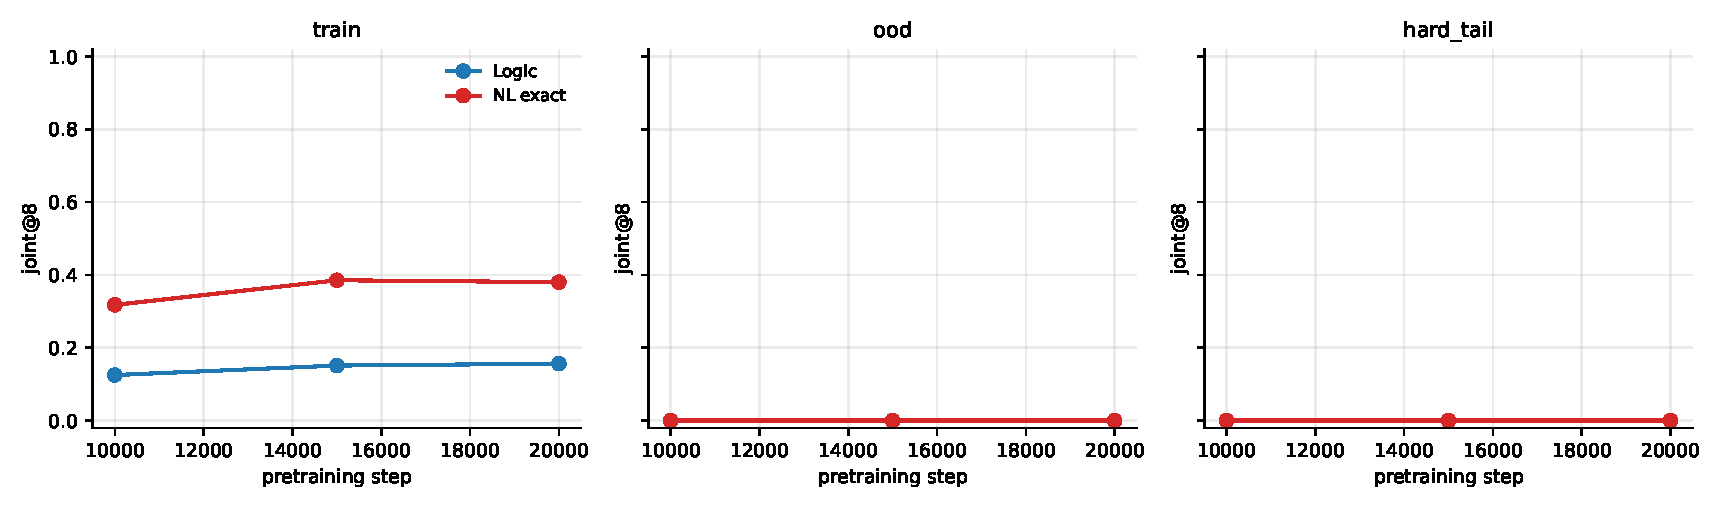
\includegraphics[width=\linewidth]{figures/tiny_llama_200m_checkpoint_joint_k8.pdf}
\caption{Tiny Llama 200m seed-mean checkpoint curves for joint correct+valid@8.}
\end{figure}

\begin{figure}[H]\centering
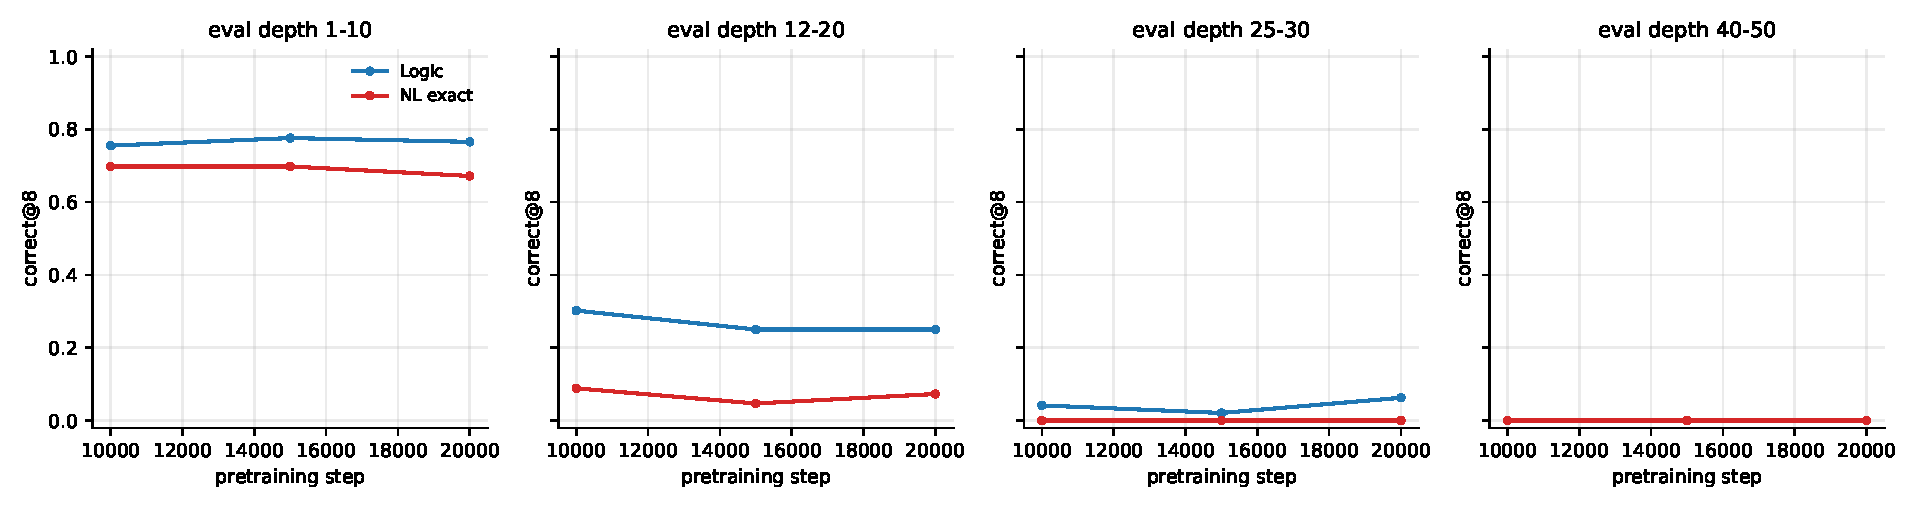
\includegraphics[width=\linewidth]{figures/tiny_llama_50m_checkpoint_depthbands_correct_k8.pdf}
\caption{Tiny Llama 50m optimizer-step curves for correct@8 over eval-depth bands.}
\end{figure}
\begin{figure}[H]\centering
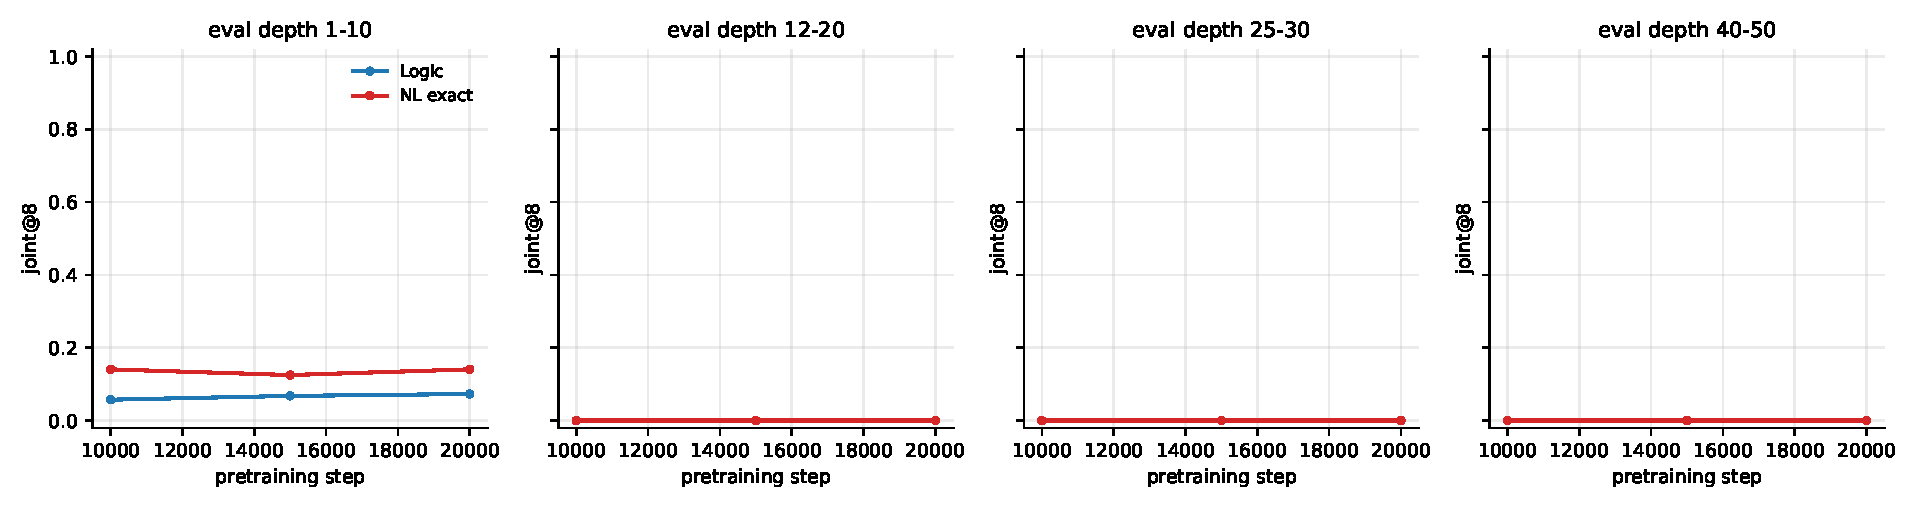
\includegraphics[width=\linewidth]{figures/tiny_llama_50m_checkpoint_depthbands_joint_k8.pdf}
\caption{Tiny Llama 50m optimizer-step curves for joint correct+valid@8 over eval-depth bands.}
\end{figure}
\begin{figure}[H]\centering
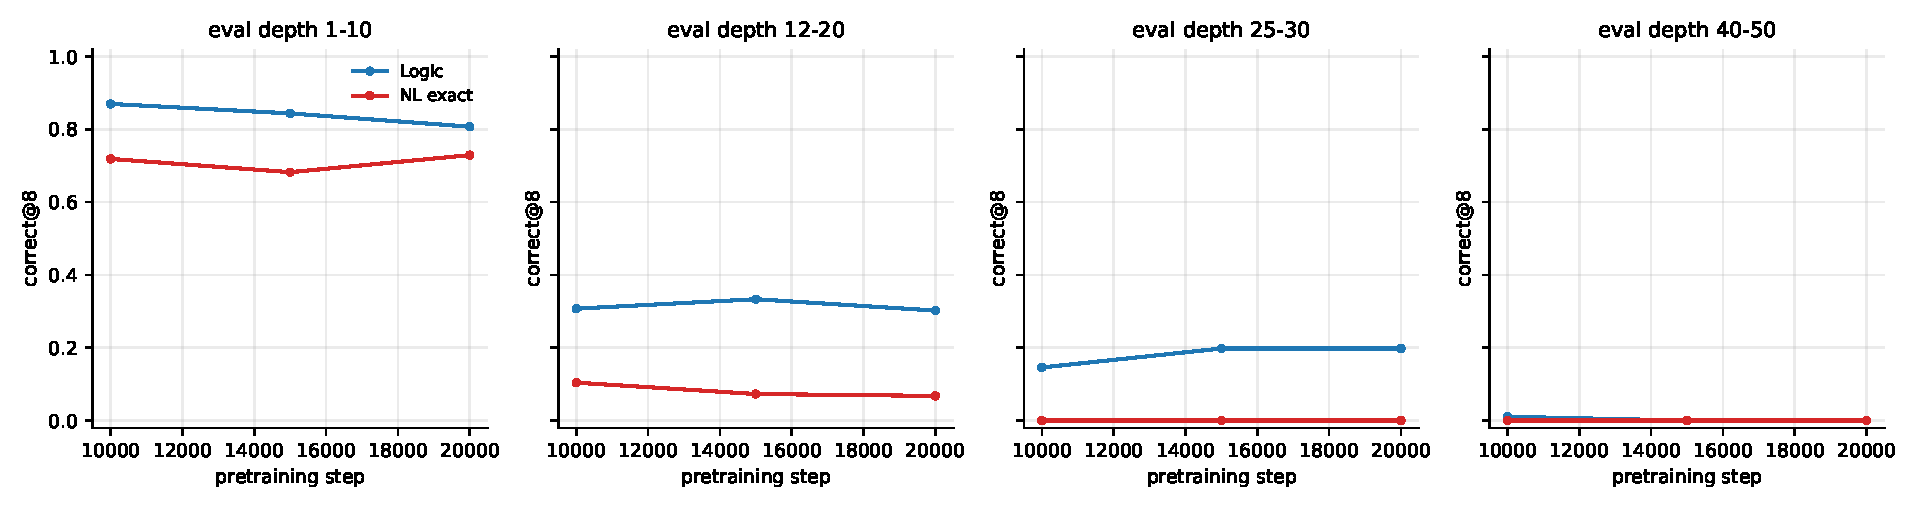
\includegraphics[width=\linewidth]{figures/tiny_llama_100m_checkpoint_depthbands_correct_k8.pdf}
\caption{Tiny Llama 100m optimizer-step curves for correct@8 over eval-depth bands.}
\end{figure}
\begin{figure}[H]\centering
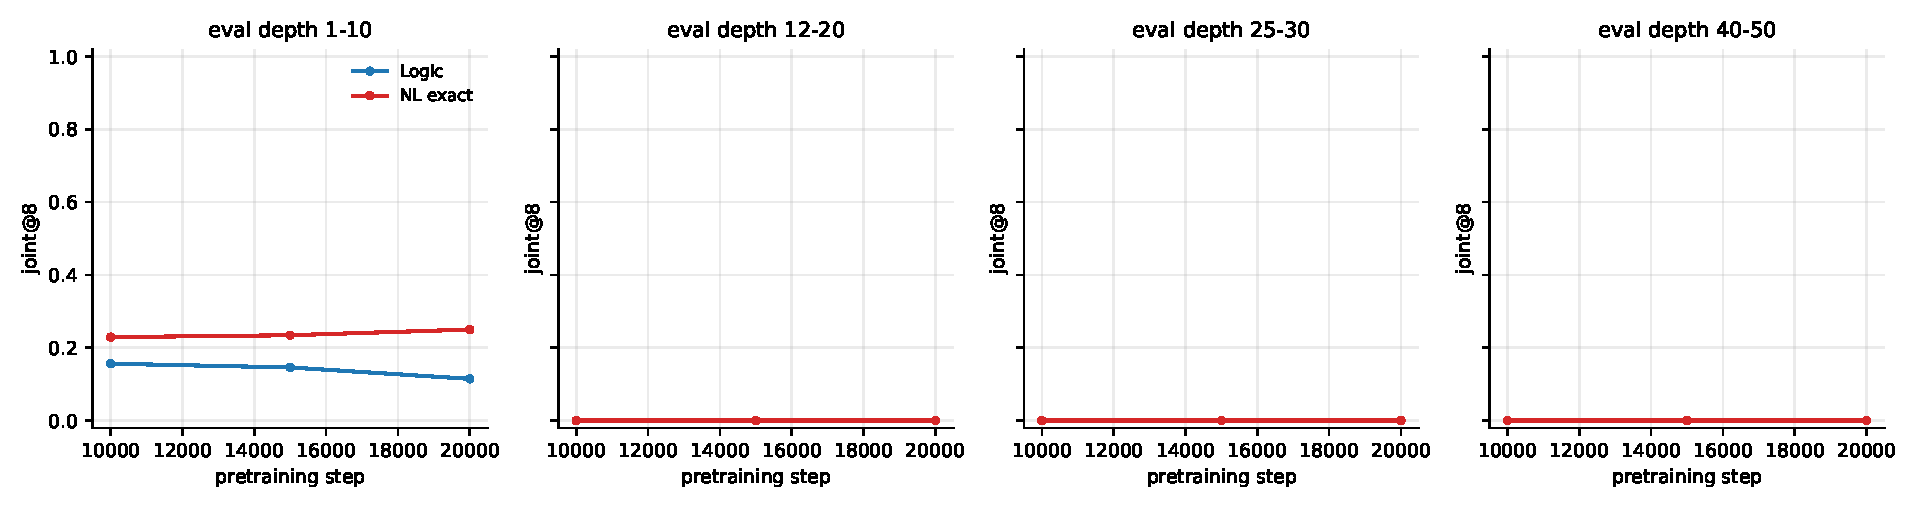
\includegraphics[width=\linewidth]{figures/tiny_llama_100m_checkpoint_depthbands_joint_k8.pdf}
\caption{Tiny Llama 100m optimizer-step curves for joint correct+valid@8 over eval-depth bands.}
\end{figure}
\begin{figure}[H]\centering
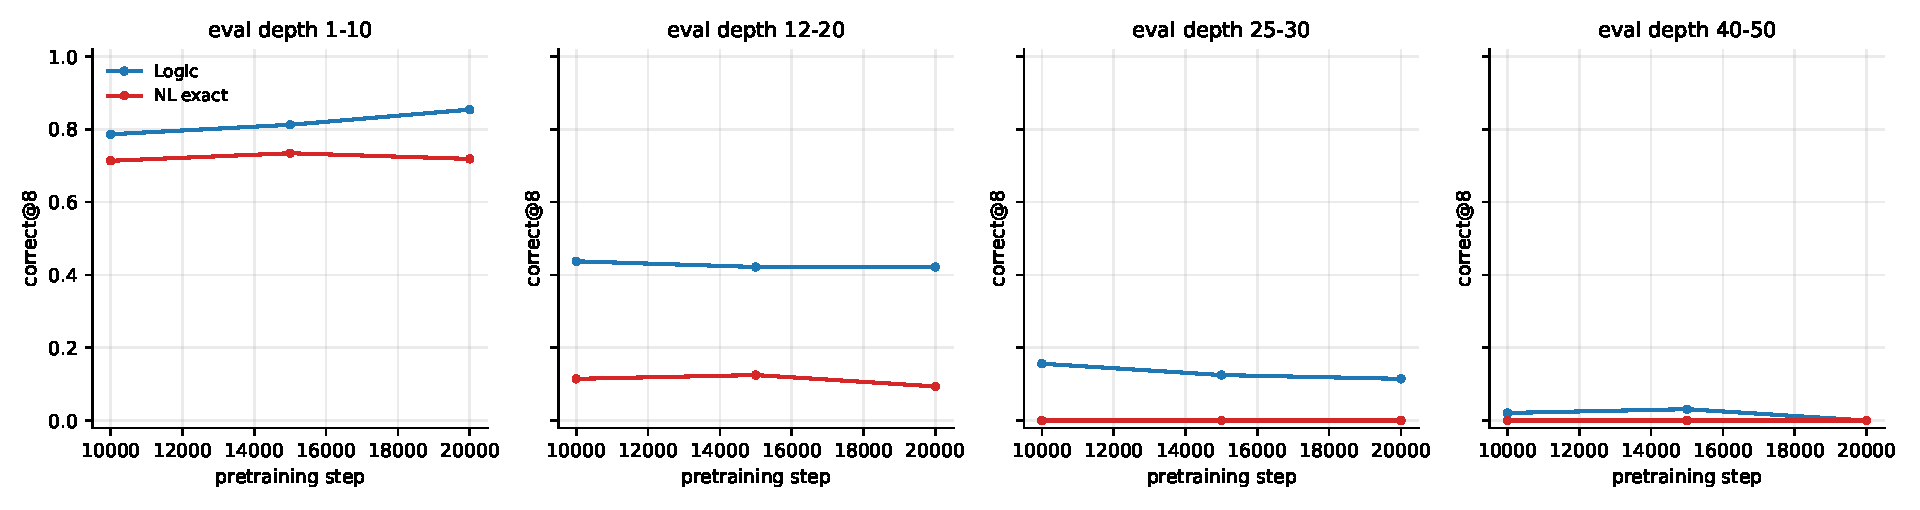
\includegraphics[width=\linewidth]{figures/tiny_llama_200m_checkpoint_depthbands_correct_k8.pdf}
\caption{Tiny Llama 200m optimizer-step curves for correct@8 over eval-depth bands.}
\end{figure}
\begin{figure}[H]\centering
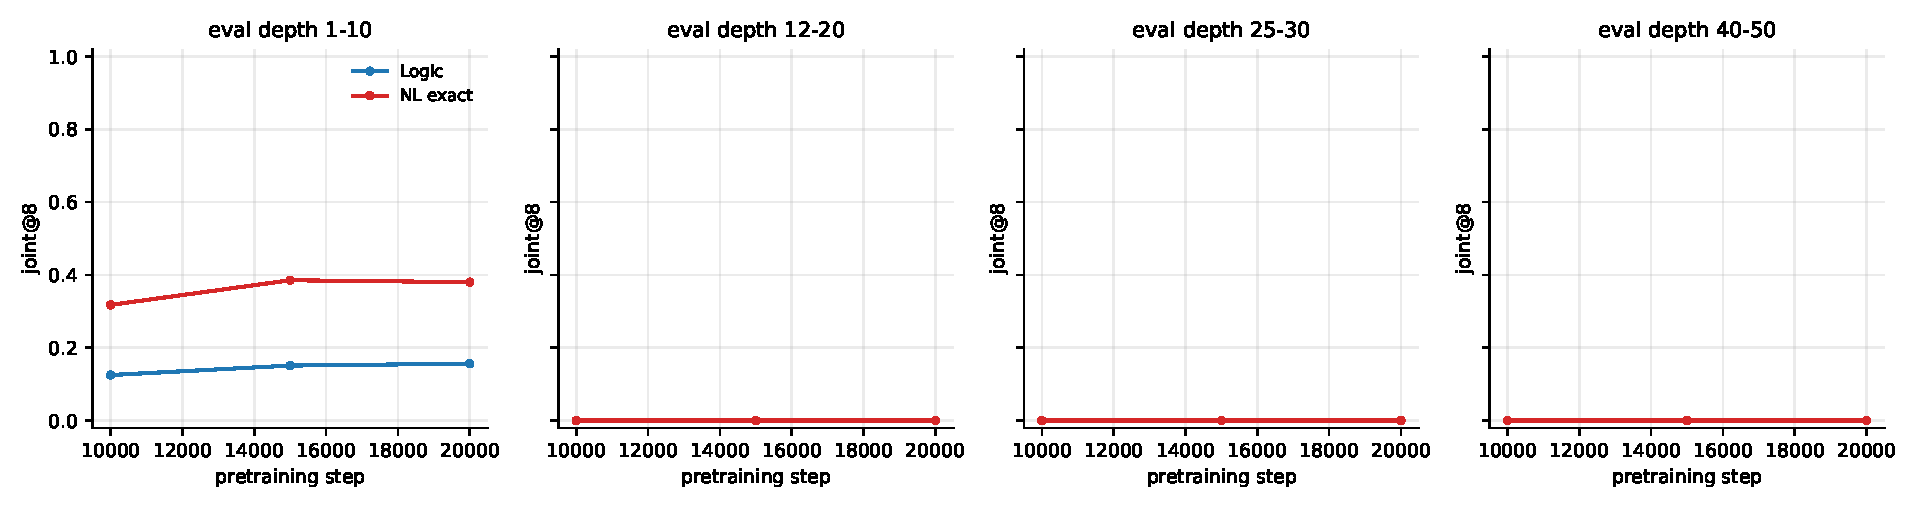
\includegraphics[width=\linewidth]{figures/tiny_llama_200m_checkpoint_depthbands_joint_k8.pdf}
\caption{Tiny Llama 200m optimizer-step curves for joint correct+valid@8 over eval-depth bands.}
\end{figure}

\subsection{Tiny Llama downstream OOD eval}
The tiny downstream OOD evals completed with the 8192-context fallback. LongBench contexts are truncated for these tiny models, so these tables are smoke/result-sanity readouts rather than fair long-context QA claims.

\begin{table}[H]
\centering
\small
\begin{tabular}{llllllll}
\toprule
size & template & n & GSM8K EM & GSM8K tag & Hotpot EM & 2Wiki EM & MuSiQue EM \\
\midrule
50m & logic & 3 & 0.000 & 0.004 & 0.000 & 0.000 & 0.000 \\
50m & nl\_exact & 3 & 0.000 & 0.029 & 0.000 & 0.000 & 0.000 \\
100m & logic & 3 & 0.000 & 0.010 & 0.000 & 0.000 & 0.000 \\
100m & nl\_exact & 3 & 0.000 & 0.055 & 0.000 & 0.000 & 0.000 \\
200m & logic & 3 & 0.000 & 0.215 & 0.000 & 0.000 & 0.000 \\
200m & nl\_exact & 3 & 0.000 & \textbf{0.403} & 0.000 & 0.000 & 0.000 \\
\bottomrule
\end{tabular}
\caption{Tiny Llama OOD exact-match metrics after strict answer extraction.}
\end{table}

\begin{table}[H]
\centering
\small
\begin{tabular}{llllll}
\toprule
size & template & n & Hotpot F1 & 2Wiki F1 & MuSiQue F1 \\
\midrule
50m & logic & 3 & 0.000 & 0.000 & 0.000 \\
50m & nl\_exact & 3 & 0.000 & 0.000 & 0.000 \\
100m & logic & 3 & 0.000 & 0.000 & 0.000 \\
100m & nl\_exact & 3 & 0.000 & 0.000 & 0.000 \\
200m & logic & 3 & 0.000 & 0.000 & 0.000 \\
200m & nl\_exact & 3 & 0.000 & 0.000 & 0.000 \\
\bottomrule
\end{tabular}
\caption{Tiny Llama OOD F1 metrics after strict answer extraction. GSM8K is omitted because it is scored by numeric exact match.}
\end{table}

\subsection{Tiny Llama bare-format OOD reruns}
Both the 20k and 100k tiny bare-format OOD arrays completed. All strict EM/F1 values remain zero on GSM8K and LongBench; the only movement is answer-tag adherence, mostly in the 200M checkpoints.

\begin{table}[H]
\centering
\small
\begin{tabular}{llllllll}
\toprule
size & template & n & GSM8K EM & GSM8K tag & Hotpot EM & 2Wiki EM & MuSiQue EM \\
\midrule
50m & logic & 3 & 0.000 & 0.026 & 0.000 & 0.000 & 0.000 \\
50m & nl\_exact & 3 & 0.000 & 0.174 & 0.000 & 0.000 & 0.000 \\
100m & logic & 3 & 0.000 & 0.084 & 0.000 & 0.000 & 0.000 \\
100m & nl\_exact & 3 & 0.000 & 0.102 & 0.000 & 0.000 & 0.000 \\
200m & logic & 3 & 0.000 & \textbf{0.822} & 0.000 & 0.000 & 0.000 \\
200m & nl\_exact & 3 & 0.000 & 0.461 & 0.000 & 0.000 & 0.000 \\
\bottomrule
\end{tabular}
\caption{Tiny Llama 20k bare-format OOD exact-match metrics.}
\end{table}

\begin{table}[H]
\centering
\small
\begin{tabular}{llllllll}
\toprule
size & template & n & GSM8K EM & GSM8K tag & Hotpot EM & 2Wiki EM & MuSiQue EM \\
\midrule
50m & logic & 3 & 0.000 & 0.017 & 0.000 & 0.000 & 0.000 \\
50m & nl\_exact & 3 & 0.000 & 0.100 & 0.000 & 0.000 & 0.000 \\
100m & logic & 3 & 0.000 & 0.069 & 0.000 & 0.000 & 0.000 \\
100m & nl\_exact & 3 & 0.000 & 0.046 & 0.000 & 0.000 & 0.000 \\
200m & logic & 3 & 0.000 & \textbf{0.675} & 0.000 & 0.000 & 0.000 \\
200m & nl\_exact & 3 & 0.000 & 0.357 & 0.000 & 0.000 & 0.000 \\
\bottomrule
\end{tabular}
\caption{Tiny Llama 100k bare-format OOD exact-match metrics.}
\end{table}

\section{Qwen-2.5-7B architecture ablation}
\begin{table}[H]
\centering
\small
\begin{tabular}{lllllll}
\toprule
template & train max & n & OOD c@16 & OOD joint@16 & d50 c@16 & d50 joint@16 \\
\midrule
logic & 10 & 3 & 0.618 & 0.320 & 0.292 & 0.031 \\
logic & 20 & 3 & 0.753 & 0.165 & 0.656 & 0.021 \\
logic & 25 & 3 & 0.906 & 0.431 & 0.854 & 0.156 \\
nl\_exact & 10 & 3 & 0.461 & 0.279 & 0.427 & 0.000 \\
nl\_exact & 20 & 3 & 0.438 & 0.339 & 0.333 & 0.135 \\
nl\_exact & 25 & 3 & 0.569 & 0.565 & 0.250 & 0.229 \\
\bottomrule
\end{tabular}
\caption{Qwen-2.5-7B representative sparse eval. This 18-row architecture slice is complete.}
\end{table}
\begin{figure}[H]\centering
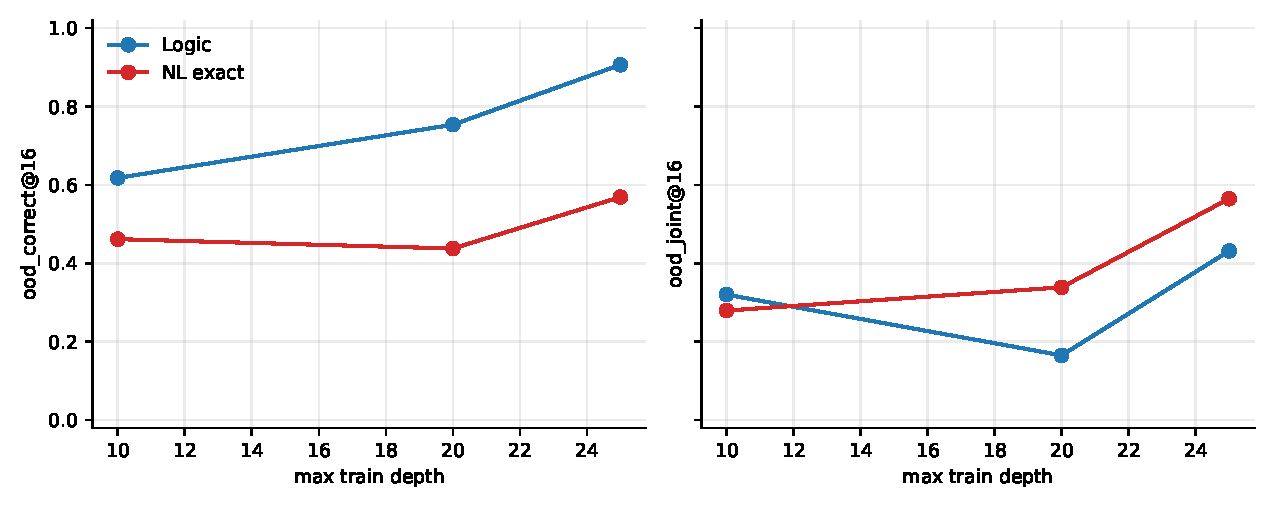
\includegraphics[width=0.86\linewidth]{figures/qwen7b_partial_ood_correct_joint.pdf}
\caption{Partial Qwen-2.5-7B OOD correct/joint@16.}
\end{figure}

\section{Targeted ablations}
Completed ablation results are shown here; active arrays are tracked in the handoff documents. The same-token-budget control keeps the logic-vs-NL comparison favorable to logic on answer correctness but not on joint validity. The shortcut-rate table currently covers shortcut rate 0.5; shortcut rate 0.8 eval rows are still running. Conditioned dual-modality eval is partial and should not be interpreted until all 30 eval rows complete.

\begin{table}[H]
\centering
\small
\begin{tabular}{lllllll}
\toprule
template & steps & n & OOD c@16 & OOD joint@16 & d50 c@16 & d50 joint@16 \\
\midrule
logic & 10000 & 3 & 0.898 & 0.335 & 0.792 & 0.125 \\
nl\_exact & 7140 & 3 & 0.554 & 0.473 & 0.344 & 0.219 \\
\bottomrule
\end{tabular}
\caption{Same target-token budget control, train-1-to-25, three seeds.}
\end{table}
\begin{figure}[H]\centering
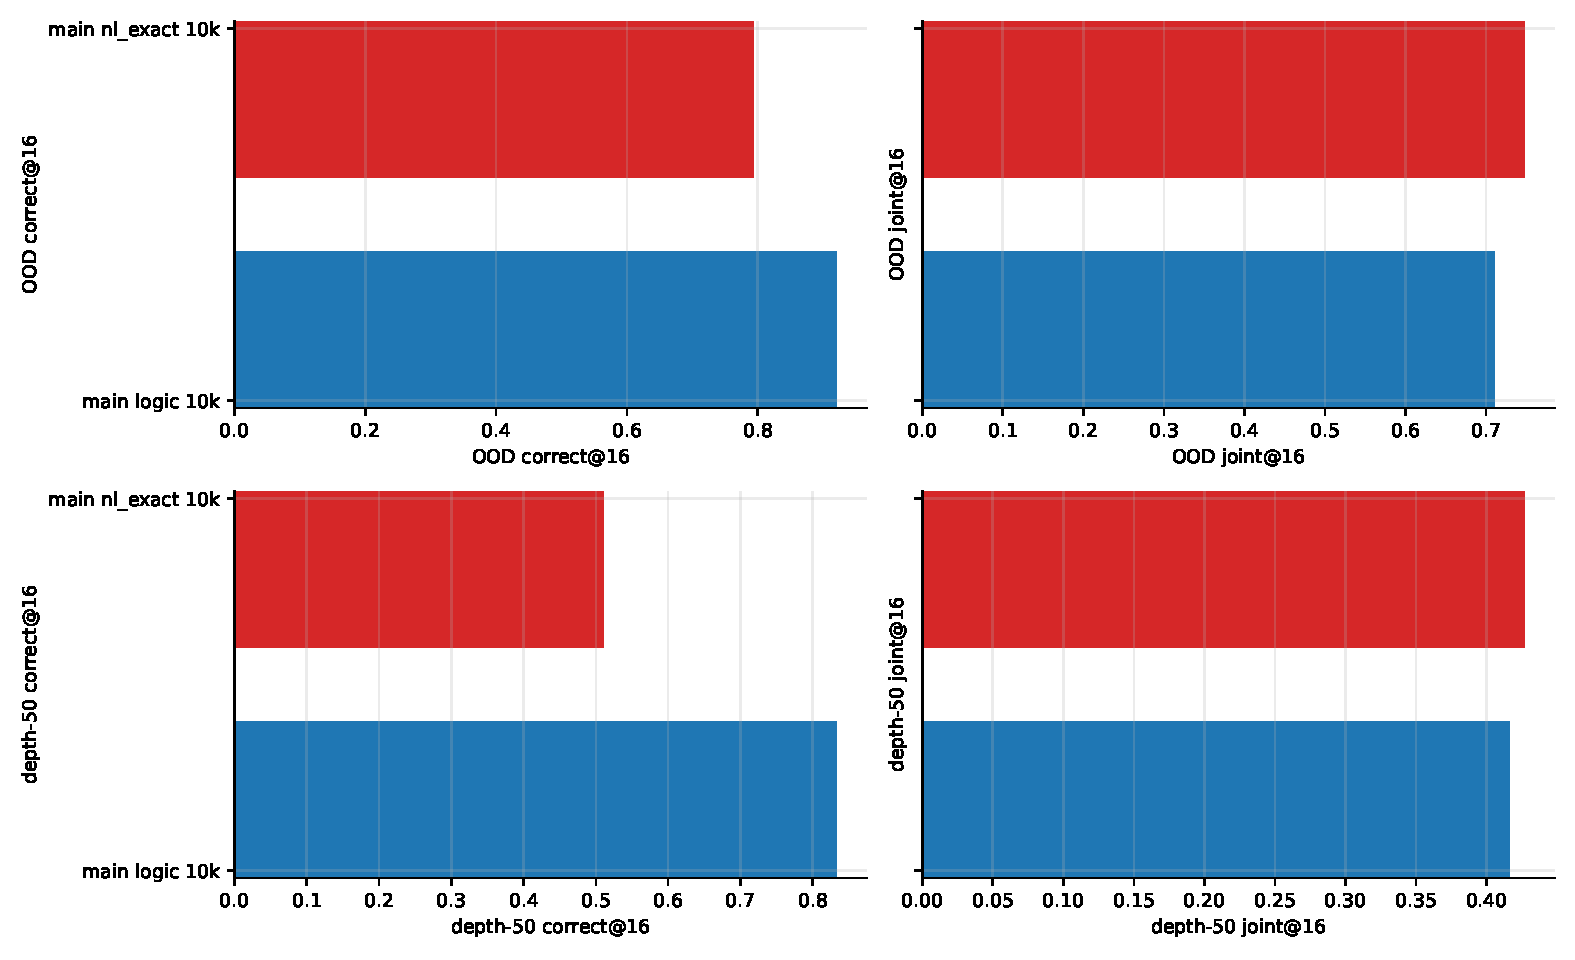
\includegraphics[width=\linewidth]{figures/ablation_same_target_token_budget_vs_main.pdf}
\caption{Same target-token budget control compared against the main train-1-to-25 logic/NL baselines.}
\end{figure}

\begin{table}[H]
\centering
\small
\begin{tabular}{lllllll}
\toprule
template & shortcut rate & n & OOD c@16 & OOD joint@16 & d50 c@16 & d50 joint@16 \\
\midrule
logic & 0p5 & 3 & 0.906 & 0.677 & 0.833 & 0.375 \\
nl\_exact & 0p5 & 3 & 0.642 & 0.585 & 0.385 & 0.312 \\
\bottomrule
\end{tabular}
\caption{Shortcut-rate ablation results available so far. Eval remains shortcut-neutral.}
\end{table}
\begin{figure}[H]\centering
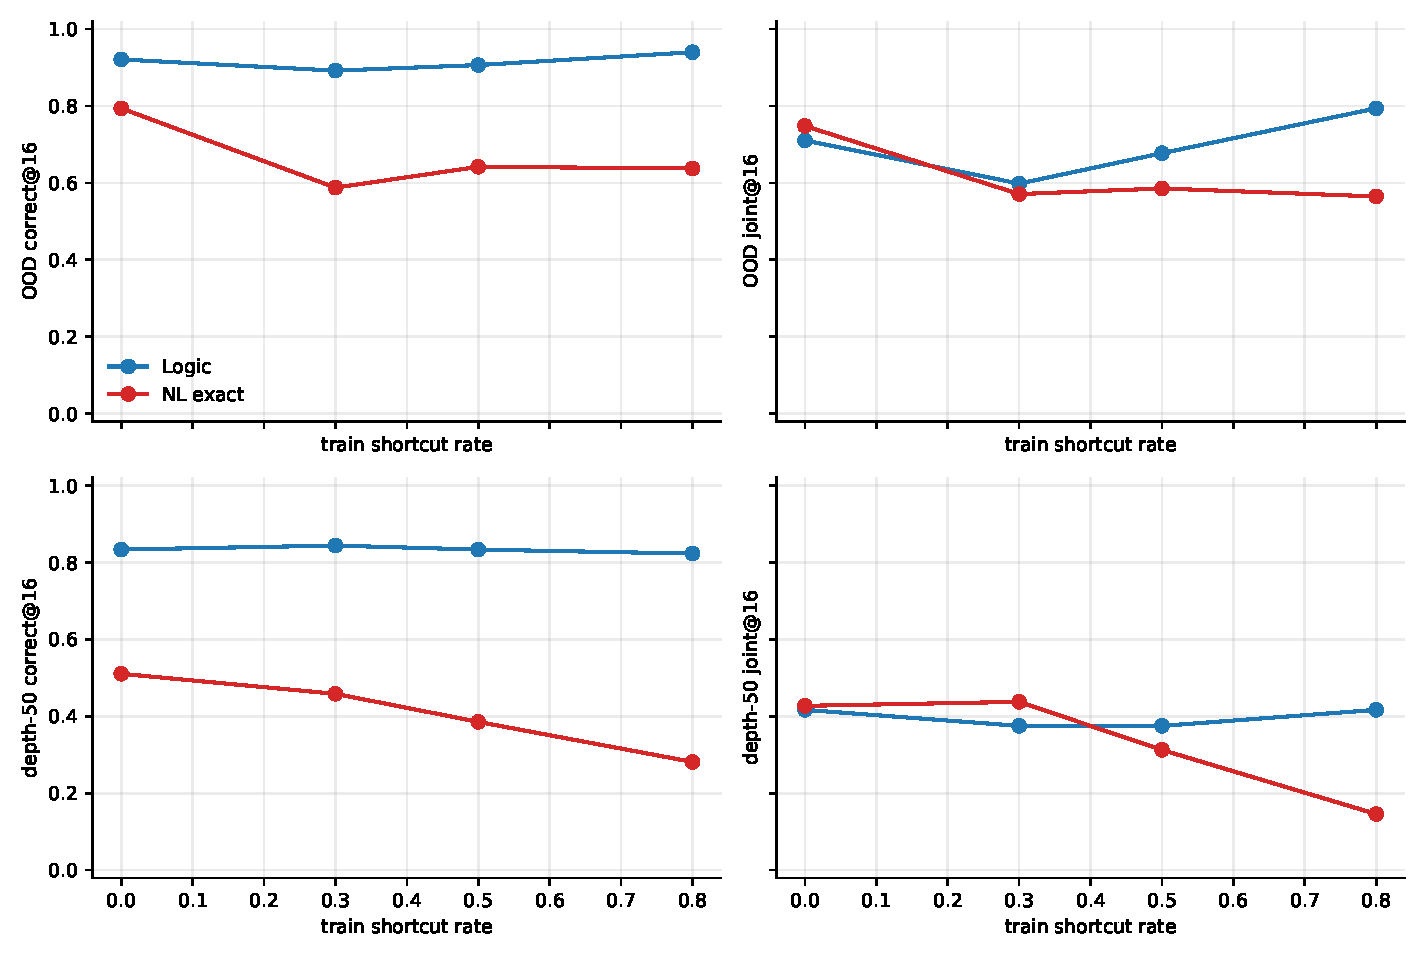
\includegraphics[width=0.9\linewidth]{figures/ablation_shortcut_rate_vs_main.pdf}
\caption{Shortcut-rate ablation compared with shortcut-neutral main train-1-to-25 baselines.}
\end{figure}

\begin{table}[H]
\centering
\scriptsize
\begin{tabular}{lllllll}
\toprule
train max & eval mode & n & OOD c@16 & OOD joint@16 & d50 c@16 & d50 joint@16 \\
\midrule
10 & conditioned\_logic & 3 & 0.695 & 0.256 & 0.521 & 0.000 \\
10 & conditioned\_nl & 3 & 0.638 & 0.339 & 0.604 & 0.000 \\
15 & conditioned\_logic & 3 & 0.572 & 0.258 & 0.344 & 0.031 \\
15 & conditioned\_nl & 1 & 0.469 & 0.191 & 0.500 & 0.000 \\
20 & conditioned\_logic & 3 & 0.701 & 0.116 & 0.500 & 0.021 \\
25 & conditioned\_logic & 3 & 0.677 & 0.202 & 0.521 & 0.031 \\
5 & conditioned\_logic & 3 & 0.360 & 0.058 & 0.167 & 0.000 \\
5 & conditioned\_nl & 3 & 0.697 & 0.332 & 0.646 & 0.000 \\
\bottomrule
\end{tabular}
\caption{Conditioned dual-modality ablation rows available at report generation time.}
\end{table}

\section{Qualitative samples}
The companion PDF \texttt{figures/sample\_generation\_panels.pdf} contains synthetic generated examples with extracted answer, gold answer, correctness, and validity metadata. The following samples are from the completed bare-format OOD rerun for OLMo-7B train-1-to-25 seed 3407.

\subsection*{gsm8k doc 3}
\textbf{Question.} James decides to run 3 sprints 3 times a week. He runs 60 meters each sprint. How many total meters does he run a week?

\textbf{Gold.} 540

\textbf{Logic extracted:}  (EM=0.000)
\begin{verbatim}
<formal>
<constants>
a = 3
b = 60
</constants>
<predicates>
Ax: x is a sprint
Bx: x is a week
Cx: x is a meter
Dx: x is a run
Ex: x is a time
Fx: x is a distance
Gx: x is a number
Hx: x is a total
Ix: x is a run time
Jx: x is a sprint time
Kx: x is a sprint
Lx: x is a week time
Mx: x is a distance run
Nx: x is a sprint distance
Ox: x is a run distance
Px: x is a sprint distance run
Qx: x is a run distance run
Rx: x is a sprint distance run
Sx: x
...[truncated]...
La
Ma
Ja
Ka
La
Ma
Ja
Ka
La
Ma
Ja
Ka
La
Ma
Ja
Ka
La
Ma
Ja
Ka
La
Ma
Ja
Ka
La
Ma
Ja
Ka
La
Ma
Ja
Ka
La
Ma
Ja
Ka
La
Ma
Ja
Ka
La
Ma
Ja
Ka
La
Ma
Ja
Ka
La
Ma
Ja
Ka
La
Ma
Ja
Ka
La
Ma
Ja
Ka
La
Ma
Ja
Ka
La
Ma
Ja
Ka
La
Ma
Ja
Ka
La
Ma
Ja
Ka
La
Ma
Ja
Ka
La
Ma
Ja
Ka
La
Ma
Ja
Ka
La
Ma
Ja
Ka
La
Ma
Ja
Ka
La
Ma
Ja
Ka
La
Ma
Ja
Ka
La
Ma
Ja
Ka
La
Ma
Ja
Ka
La
Ma
Ja
Ka
La
Ma
Ja
Ka
La
Ma
Ja
Ka
La
Ma
Ja
Ka
La
Ma
Ja
Ka
La
Ma
Ja
Ka
La
Ma
Ja
Ka
La
Ma
Ja
Ka
La
Ma
Ja
Ka
La
Ma
\end{verbatim}
\textbf{NL extracted:} 540 (EM=1.000)
\begin{verbatim}
<think>
<premises>
a = 3
b = 3
c = 60
</premises>
<proof>
a = 3
b = 3
c = 60
total = a * b * c
total = 3 * 3 * 60
total = 540
</proof>
<conclusion>
James runs 540 meters a week.
</conclusion>
</think>
<answer>
540
\end{verbatim}

\subsection*{hotpotqa doc 0}
\textbf{Question.} Question: Which case was brought to court first Miller v. California or Gates v. Collier ?

\textbf{Gold.} Miller v. California

\textbf{Logic extracted:} Gates v. Collier (F1=0.333)
\begin{verbatim}
<answer>
Gates v. Collier
\end{verbatim}
\textbf{NL extracted:}  (F1=0.000)
\begin{verbatim}
<think>
<premises>
austrian supplier Gasser and Italian distributor MISAT entered into a contract together for the supply of children's clothes. In the contract, they included a choice-of-court agreement, stipulating that an Austrian court have jurisdiction in case of conflict. However, when a dispute arose between the two parties, MISAT seised an Italian court to declare that the contract had been terminated, contrary to the choice-of-court clau
...[truncated]...
ending the choice-of-court agreement experience substantive disadvantages in the other Member State, as the court situated there might declare the agreement invalid, the party may also be exposed to procedural disadvantages, caused by judicial system which is not chosen.: 573  This in turn can make the jurisdiction agreement ineffective altogether, going against the principle of party autonomy. Taking a formalistic and literal approach, the Court
\end{verbatim}

\subsection*{2wikimqa doc 0}
\textbf{Question.} Question: Where was the wife of Francis I Rákóczi born?

\textbf{Gold.} Ozalj

\textbf{Logic extracted:} Ozalj (F1=1.000)
\begin{verbatim}
<answer>
Ozalj
\end{verbatim}
\textbf{NL extracted:} Ozalj (F1=1.000)
\begin{verbatim}
<answer>
Ozalj
\end{verbatim}

\subsection*{musique doc 0}
\textbf{Question.} Question: Who plays the wife of the producer of Here Comes the Boom in Grown Ups?

\textbf{Gold.} Maria Bello

\textbf{Logic extracted:} Maria Bello (F1=1.000)
\begin{verbatim}
<answer>
Maria Bello
\end{verbatim}
\textbf{NL extracted:}  (F1=0.000)
\begin{verbatim}
<think>
<premises>
aikido
aikido
aikido
aikido
aikido
aikido
aikido
aikido
aikido
aikido
aikido
aikido
aikido
aikido
aikido
aikido
aikido
aikido
aikido
aikido
aikido
aikido
aikido
aikido
aikido
aikido
aikido
aikido
aikido
aikido
aikido
aikido
aikido
aikido
aikido
aikido
aikido
aikido
aikido
aikido
aikido
aikido
aikido
aikido
aikido
aikido
aikido
aikido
aikido
aikido
aikido
aikido
aikido
aikido
aikido
aikido
aikido
aikido
aikido
aikido
aikido
aiki
...[truncated]...
aikido
aikido
aikido
aikido
aikido
aikido
aikido
aikido
aikido
aikido
aikido
aikido
aikido
aikido
aikido
aikido
aikido
aikido
aikido
aikido
aikido
aikido
aikido
aikido
aikido
aikido
aikido
aikido
aikido
aikido
aikido
aikido
aikido
aikido
aikido
aikido
aikido
aikido
aikido
aikido
aikido
aikido
aikido
aikido
aikido
aikido
aikido
aikido
aikido
aikido
aikido
aikido
aikido
aikido
aikido
aikido
aikido
aikido
aikido
aikido
aikido
aikido
aikido
aikido
a
\end{verbatim}

\section{Artifacts}
CSV tables live under \texttt{tables/} and all plots are emitted as both PDF and PNG under \texttt{figures/}. This machine currently lacks \texttt{pdflatex}/\texttt{latexmk}, so the LaTeX source is generated but not compiled here.
\end{document}
